\documentclass{template}
\usepackage{color}
\usepackage[hyphens]{url}
\usepackage{longtable}
\usepackage{graphicx}
\usepackage{enumitem}
\usepackage{pdfpages}
\usepackage{hyperref}

\def\etal{{\it et al.~}}
\newenvironment{packed_enum}{
\begin{enumerate}
  \setlength{\itemsep}{1pt}
  \setlength{\parskip}{0pt}
  \setlength{\parsep}{0pt}
}{\end{enumerate}}
\newenvironment{packed_item}{
\begin{itemize}
  \setlength{\itemsep}{1pt}
  \setlength{\parskip}{0pt}
  \setlength{\parsep}{0pt}
}{\end{itemize}}

\begin{document}

\title{Tor's Usability for Censorship Circumvention}
\numberofauthors{1}
\author{
 \alignauthor Linda N. Lee, David Fifield, Nathan Malkin \\
   \vspace{0.5em}
   \affaddr{University of California, Berkeley} \\
   \affaddr{\{lnl,fifield,nmalkin\}@cs.berkeley.edu}\\
}
\maketitle

\begin{abstract}
Tor has grown beyond its original purpose as an anonymity tool and has 
since become an important censorship circumvention tool. It is now listed
as one of the ways that normal people use Tor \cite{whotor}.
We specifically examine its usability as a censorship circumvention tool,
an essential facet for adoption and use.  
We focus our analysis on the connection configuration interface of Tor Browser,
as censorship circumvention requires correct transport configurations.
The first phase of the study evaluated if and how easily users can circumvent censorship 
using Tor Browser; the results of conducting our experiment and the interface redesign
is presented in this paper. The second phase
of the study will test the improvements to the interface, which has yet to happen. However, we take
some time to describe our plans. 
Our goal is to integrate positive usability changes into the Tor Browser, making
censorship circumvention an easier process for users around the world. 

\end{abstract}

\keywords{Censorship, Security, User Studies, Anonymity, Tor}

\section{Introduction}
Tor is primarily known as the most widely used anonymity tool today. 
For this reason, user studies on Tor have been solely about the usability of Tor as an
anonymity tool. Norcie~\cite{norcie2012eliminating} conducted an experiment which identified 
``stopping points'' in Tor Browser, documenting points when people would get frustrated enough
to stop using Tor. To our knowledge, that has been the only published user study of Tor. 
Since then, Tor has had a lot of updates. There have been been no published usability evaluations of
Tor Browser since the introduction of the 4.0 series, which introduced radical UI changes. 
Lee and Fifield \cite {uxsprint} ran a small pilot study testing the download, install, and user interface of Tor Browser. 
This study uncovered a number of bugs and stopping points. Changes made are reflected in series 
5.1 and later. There has been no work done on Tor as a censorship circumvention tool. 

Many features of Tor have not been evaluated through user
research --- such as advanced web tasks (e.g., accessing hidden services), the
configuration menu to connect to the Tor network, configuring automatic
updates, and identity/cookie management. Rather than selecting the features to
study in isolation, we decided to focus on an important use case of Tor browser: censorship circumvention. 
Internet censorship is pervasive across the world today \cite{faris2008measuring}. 
Although Tor was not designed to be a censorship circumvention tool, users started
using it as one, since Tor's role as a proxy to anonymize
people also worked to circumvent censorship. Now, circumventing censorship is a
common use case for Tor, and current censorship circumvention methods are
incorporated into Tor, making it a viable censorship circumvention tool even in the face
of adversaries. In fact, some countries unsuccessfully attempt to block Tor for this reason \cite{winter2012great}. 
To our knowledge, this is the first user study investigating the usability of Tor as a 
censorship circumvention tool.

We believe that this is a great opportunity for user research. Censorship circumvention
is not only a common use case, but one Tor was not intended for. Tor does not
track their users in any way or perform A/B testing, making a user study a more
uniquely beneficial source of feedback. Since the interface does not depend on the 
internal functionality of Tor, changes made to the configuration interface would not
require huge changes, making any suggested improvements very practical to 
deploy. 

\section{The Configuration Interface}

\noindent {\bfseries Overview}
The Tor Browser provides a configuration interface to guide users through setting up 
their connection to the
Tor network. While most can connect to Tor using the
dialog's default settings, users in certain censorship environments must
make use of additional settings, such as bridges, proxies, or both. 
Our study explores how the average user circumvents censorship
through this interface.

For context, we will give the definition of bridges, pluggable transports, and proxies. 
Keep in mind that this is the kind of information that a user might need to know to be able
to configure correctly. Note that bridges, pluggable transports, and proxies are technical 
concepts which may be unfamiliar to the average user, and that bridges and pluggable
transports are completely Tor-specific concepts. 

Bridges are unlisted Tor relays that make it possible for a user to connect
to the Tor network even if a censor blocks all publicly listed Tor relays. There used 
to be plain relays which were exactly similar to public relays, but were unlisted. However, 
censors in countries which blocked Tor generally were motivated enough to aggressively
block Tor in other ways, such as traffic analysis. For this reason, a bridge is usually associated
with a pluggable transport that circumvents deep packet inspection. Transports can
assist by obfuscating traffic or reflecting traffic through a content distribution network. 
Proxies help bypass local network restrictions and are typically only
needed in restricted cases, such as corporate environments.\\

\noindent {\bfseries Configuration Flow}

\begin{figure*}[t]
  \centering
    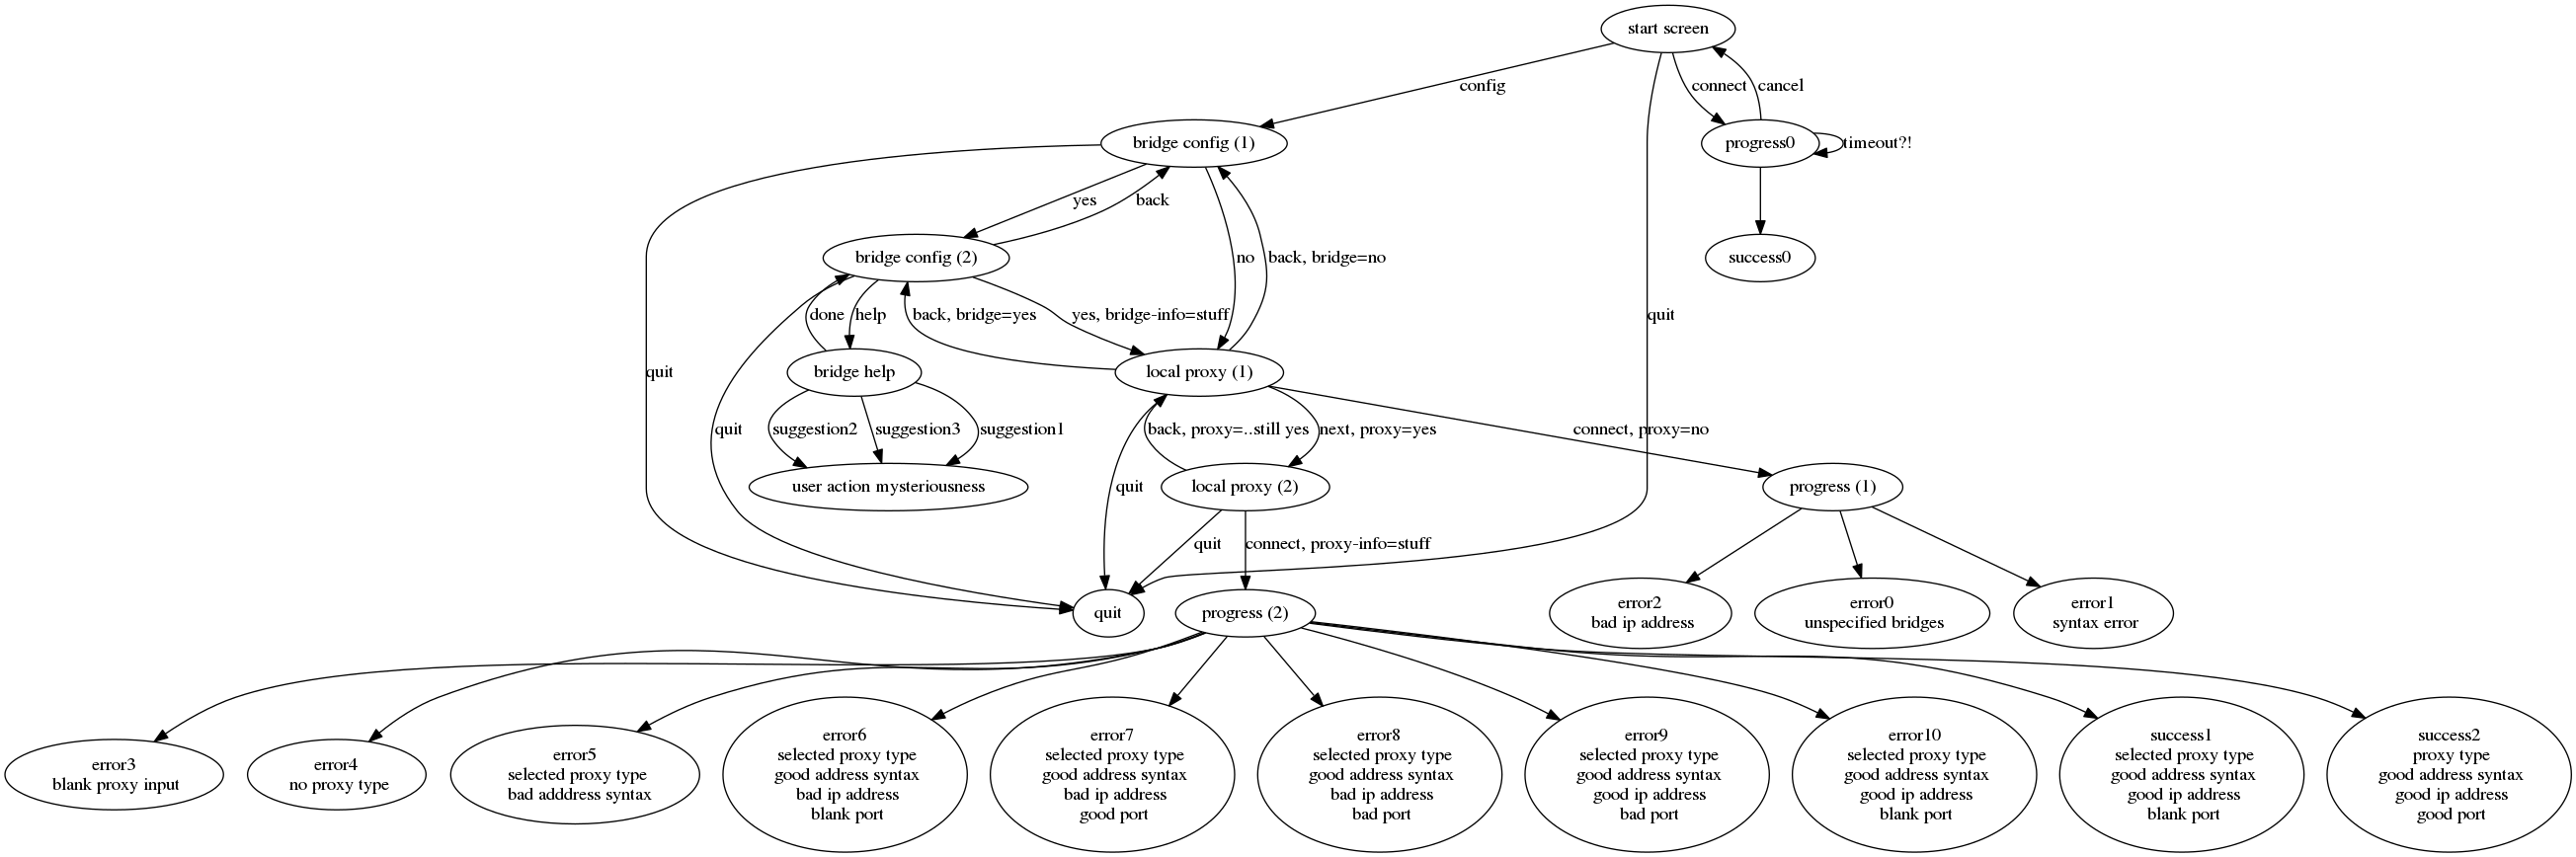
\includegraphics[width=\textwidth]{../torconfig.png}
    \caption{This flow chart shows all of the possible paths taken through the
    Tor configuration interface. A state represents a window in the interface,
    with the exception of the leaves, which indicate the final action taken by
    the interface (``q'' for quit, ``s'' for success, and ``e'' for error). The
    transitions between the states indicate which user action causes that
    transition. Annotations for the error states can be found by following
\href{https://github.com/lindanlee/circumvention-ux-tor/blob/master/torconfig.dot}{this hyperlink}.}
\label{fig:interface}
\end{figure*}

As bridges and proxies can be configured independently or together, there are
four main ways to set up a connection:

\begin{enumerate} \itemsep1pt \parskip0pt \parsep0pt
    \item With a bridge and proxy
    \item With a bridge but no proxy
    \item Without a bridge but with a proxy
    \item Without either a bridge or proxy
\end{enumerate}

The launcher interface asks a series of questions to
determine which of these configuration states a user requires.
The four high-level states correspond to five distinct paths through the
configuration interface. (The latter option -- connecting with neither a bridge
nor proxy -- contributes two separate paths.) Each path branches further
depending on user-specific inputs. Figure \ref{fig:interface} illustrates the
resulting paths. 

When the configuration window opens, a user is given the option to connect
directly to the Tor network by clicking ``Connect'', or to click ``Configure''
``if this computer's Internet connection is censored or proxied'' (Figure
\ref{fig:window1}).

If they choose the latter, the next screen asks, ``Does your Internet Service
Provider (ISP) block or otherwise censor connection to the Tor network?''
(Figure \ref{fig:window2}). Though this sounds repetitive, it is meant to
identify and divert users who need only a proxy (and no bridge).
This phrasing of the question carries the assumption that people will
not know if they need a bridge or not, but that they are equipped to answer if their
current network environment censors the Tor Network. 

\begin{figure}[t]
\label{fig:bridges}
  \centering
    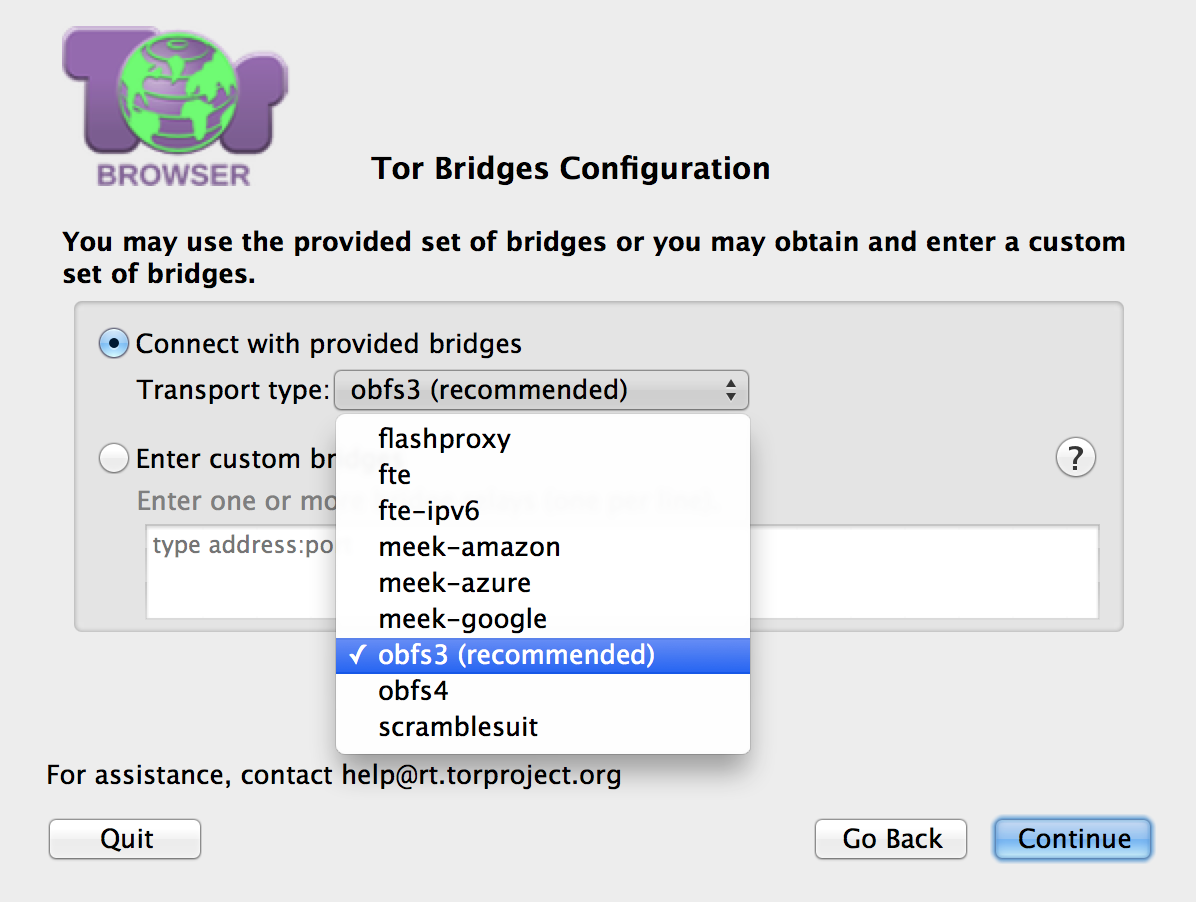
\includegraphics[width=0.5\textwidth]{configuration-screenshot.png}
    \caption{The Tor Bridges Configuration window of the Tor configuration
    interface.}
\label{fig:bridges}
\end{figure}

Next, users are asked to configure bridges by selecting a transport type from a
dropdown menu or entering the IP address of a custom bridge in a textbox (Figure
\ref{fig:bridges}).
Finally, users are asked whether they need a local proxy (Figure
\ref{fig:window4}) and (if they answered yes) to configure it (Figure
\ref{fig:window5}).

Note that a user can decide to click ``Configure'' on the first screen, but then
opt out of both bridges and proxies.
In this case, connecting after these configuration steps
would be equivalent to clicking ``Connect'' on the first screen. \\ 

\noindent {\bfseries Design choices}
The launcher interface utilizes a number of techniques to aid users and simplify
the choices they have to make. Help buttons and a support email address that
appears on every screen are meant to assist users that get stuck in the process.
The interface also makes good use of defaults, for example by emphasizing that
certain options ``will work in most situations.''

Still, there remains potential for confusion, especially with the more advanced
configuration options.
Bridges, pluggable transports, and proxies are never defined for the user,
arguably because they might not read or understand these definitions.
This can lead to users confusing these terms, or not understanding
the relations between them. Additionally, there is limited explanation of 
what pluggable transport types to choose from if the default one fails or how to 
find proxy settings, which will be required of some users. 

\section{Hypotheses}
We expected that the average user will struggle to connect because they do not understand censorship circumvention or the  censorship circumvention technologies offered by Tor. We also predict that a user will not get the feedback they need to revise their connection configuration if they fail. Specifically: 

\begin{itemize} \itemsep1pt \parskip0pt \parsep0pt
\item  {\bfseries Hypothesis 1}: users will generally not know when they need a bridge or proxy, leading to issues such as choosing to configure a bridge or proxy when it is not necessary, or configuring bridges or proxies incorrectly.
\item  {\bfseries Hypothesis 2}: people will not know when they need to configure or connect, since they do not understand how censorship works.   
\item  {\bfseries Hypothesis 3}: proxies will cause confusion when configuring bridges. 
\end{itemize} 

We find these hypotheses to be true for our participants, although sometimes not for the reasons we expected. For instance, we believed that proxies will cause confusion when configuring bridges because participants would confuse the two; however, the interface redirected users to proxy configuration settings if a participant had chosen to configure a proxy, even if the source of failure was not from the proxy. Details of the experiment that has verified our hypotheses is below.

\section{Methodology}

To test our hypotheses, we simulated several environments in which people may
have to use Tor for censorship circumvention. We examined whether users are able
to join the network and studied how they interact with the launcher interface.
Based on our findings, we designed improvements to the Tor launcher interface,
which we test in a large-scale study.

\subsection{Simulated censorship environments}
We simulated three censorship environments.
They are informed by our experience with pluggable transports
and knowledge of commonly seen censorship techniques.
They are not meant to perfectly replicate the network environment
in any particular country. Although inspired by reality, these
abstract simulations are intended to require distinct configurations
of the Tor Browser from our participants.

\begin{itemize} \itemsep1pt \parskip0pt \parsep0pt
\item {\bfseries Mild censorship} 
(Representative of countries such as France and Australia.)
Certain domains are blocked. Reaching these 
domains requires a censorship circumvention 
tool. The default option to ``connect'' to the Tor network 
directly will circumvent this censor. Additional correct
bridge or proxy configurations are optional. 

\item {\bfseries Intermediate censorship} 
(Representative of countries such as Tunisia.)
Certain domains are blocked. Censorship circumvention
tools such as Tor are blocked. Since all public Tor
relay nodes are blocked, the default option to ``connect'' to the Tor network
directly will fail. Any choice of a hard-coded bridge
or a valid non-public bridge will circumvent this censor.  
Additional correct proxy configuration is optional.

\item {\bfseries Comprehensive censorship} 
(Representative of countries such as China and Syria.)
Certain domains are blocked. Censorship circumvention tools
are thoroughly blocked. Tor is blocked by blocking all public
Tor relay nodes, and the censor has examined source code to block
all hard-coded bridge relays in the configuration interface. The default option
to ``connect'' to the Tor network directly will fail. Most bridges will fail,
but ``meek-amazon,'' ``meek-azure,'' and ``meek-google'' still work.
% TODO: meek-google doesn't work either, right? Should we remove it?
This is because domain-fronting requires censors to block entire CDNs to also
block this transport (which will cause huge collateral blocking damage), making
it resistant to aggressive censorship environments.
(See ~\cite{fifield2015blocking} for additional details.)\\
\end{itemize}

\subsection{Qualitative interface evaluation}
To identify problems with the existing interface, we conducted a series of
qualitative evaluations with a set of users representative of the general
population.

Using established best practices from the field of user experience research
(\cite{howmanyusers}), we recruited five users for each censorship environment.
We pre-screened our participants to have a good mix of gender, age, technical
background, and familiarity with Tor in each environment, and also overall. \\

%Some references to keep in mind when explaining:
%\href{why 5 users}{http://www.nngroup.com/articles/how-many-test-users/}
%\href{screening}{http://www.userfocus.co.uk/articles/screeners.html}
%\href{summative and usability mixed model}{http://www.usabilitybok.org/summative-usability-testing}

\noindent {\bfseries Procedure}
The experiment begins with the participants being informed that they are in a
simulated censorship
environment, where some --- but not all --- websites are blocked. We
instruct them to visit a non-blocked website and a blocked website on a
``standard'' browser (one that is not used for censorship circumvention, such
as Chrome, Internet Explorer, or Firefox) to illustrate the situation.
Participants are told that their
role is that of a regular citizen who is trying to visit blocked websites
for non-critical purposes,
and for whom the chance of risk is minimal. This information is given
to achieve
consistency across participants: behaviors may change if the tasks are
critical or if there are great risks associated with configuration mistakes.

After explaining the situation and the user's role, we
instruct them to complete a set of
tasks which will require visiting blocked websites. Ultimately, the
participants will need to configure their Tor Browser to circumvent the
simulated censorship environment. These tasks have a three-fold purpose of
providing participants with feedback (if they did not correctly configure their
browser, they cannot reach the website), motivating the participants to
configure the browser correctly, and providing the researchers with an
indicator of successful censorship circumvention.
Participants' screens are recorded to capture how they configure
their browser.

After users completed the browsing tasks (or time ran out), we conducted an
interview asking participants about their censorship circumvention experience.
We were able to tailor the interview to the particular participant, since we were able to
observe our participants' sessions. This way, we could follow up and ask participants
about reasons for taking particular actions and verify any hypothesis we had about 
the participant (such as ``they didn't know what to do on window 3'').  We did
ask a couple question across all participants: 
``What was the most challenging part of connecting?''
and
``What is one change you would recommend?''


\subsection{Interface design and iteration}
After completing the qualitative user studies, we analyzed the results to
identify common themes and problems. These were the basis of our interface 
redesign. To do this, we used an iterative design process, starting with low-fidelity
(paper and pencil) prototypes and then proceeding to higher-fidelity (realistic clickable mockups)
prototypes.

We collected feedback from researchers, professors, and Tor users and developers
through the Tor project's mailing lists. We iteratively designed by
incorporating the comments and suggestions we received into the next version of
the interface. We plan to take qualitative measurements of the new design
by having participants think aloud while they use our realistic mockup. This is
to get any feedback before we launch our quantitative interface evaluation.

\subsection{Quantitative interface evaluation}
Once the new design of the user interface is finalized, we will conduct a
large-scale quantitative evaluation, to test whether the improvements had a
measurable effect on people's ability to connect to the Tor network.

The experimental procedure will be nearly identical to the procedure for the
qualitative portion of the study, described above. However, rather than
conducting open-ended interviews at the end of the tasks, participants will be
asked to fill out a brief survey. Furthermore, the interface will be
instrumented to collect metrics and statistics for use in analysis and
hypothesis testing. Such metrics include the time spent on each screen, which
paths were taken, which interface elements were interacted with, etc.

Participants will be split across several different experimental conditions.
Some will be testing the improved user interface, while those in the control
group will be completing the same tasks using the old, unimproved interface. \\
% NOTE: removed mention of the alternate interface, unless there's something to say about it

\noindent {\bfseries Experiment Logistics} 
We plan to recruit up to 100 users for the purpose of this study,
making it the largest user study of Tor to date.  This study will be conducted at the
Experimental Social Science Laboratory (Xlab)
at the University of California, Berkeley, which consists of 36 laptops,
separated by cubicle walls. We will use individual host firewalls to simulate
censorship environments and will record computer screens to capture 
user activity. The total length of the experiment, including briefing, completing the censorship 
circumvention tasks, exit survey, and debriefing, will be about an hour.
Participants will be compensated \$30 for their time, which covers
minimum wage for an hour and any transportation costs to the lab. 
The IRB protocol to run this user study has been approved (2014-12-6995). 

\section{Initial Results}

The qualitative interface evaluation yielded hours of observations and
interview data, for a set of 16 pre-selected, diverse participants taking
various UI paths in different simulated censorship environments. This section
discusses the insights gathered from the qualitative interface evaluation, which
has shaped the re-design of the interface. All of the results are grounded in
participants' experiences and feedback, which are available publicly online. The
video screen captures from the experiment can be found
\href{https://github.com/lindanlee/circumvention-ux-tor/tree/master/sessions/pre/videos}{here};
a summary of each video can be found
\href{https://github.com/lindanlee/circumvention-ux-tor/blob/master/sessions/pre/participant-summaries.txt}{here}.
The corresponding notes from the after-experiment interview can be found
\href{https://github.com/lindanlee/circumvention-ux-tor/tree/master/sessions/pre/notes}{here}. 

In each censorship environment, we evaluated one Tor user, one who has heard of Tor before the study, and at least three people who had never heard of Tor before. Small-scale qualitative studies results in rich information about each participant, but making generalizations from these results such as ``Tor users were able to configure quicker'' would be unsound. Our observations of our particular three Tor users were that they were more capable of debugging after failure modes and were more methodological about doing so, but they faced similar difficulties as the other participants. \\

We noticed four common challenges:  

\begin{itemize} \itemsep1pt \parskip0pt \parsep0pt
\item {\bfseries Challenge 1:} People don't know how to choose between ``connect directly'' versus ``configure'' on the first screen. As seen in Figure \ref{fig:window1}, there is some guidance for the users, but we found this largely unhelpful since people do not understand the text on the screen. 
\item {\bfseries Challenge 2:} People feel compelled to set up a bridge, even if they don't need one, because they do not know how censorship works. Participants knew that they were censored to some degree since we had simulated censorship of websites. However, bridges are only necessary when the government has taken active steps to censor Tor itself.
\item {\bfseries Challenge 3:} When their first attempt to connect fails, the interface directs people to the last window they saw before the connection failure. The problem is not necessarily where the interface directs users, misguiding them. It was common for the interface to redirect users to the proxy window in Figure \ref{fig:window5}, even when they needed to pick another bridge. 
\item {\bfseries Challenge 4:} When the first attempt to connect fails, people did not know what to do or what to try next. The feedback given to users was not understood (see Figure \ref{fig:error}) and also did not guide users into specific actions (such as trying a different bridge, trying the same configuration again, try connecting directly, etc.).
\end{itemize}

\begin{figure}[t]
  \centering
    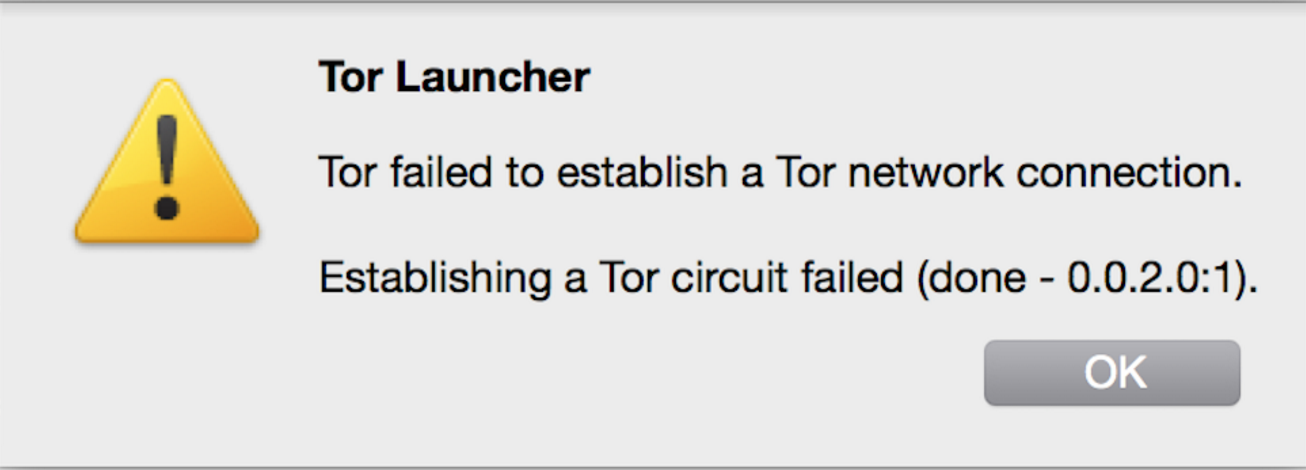
\includegraphics[width=0.5\textwidth]{error.png}
    \caption{An example of a technical error message which our participants did not understand.}
\label{fig:error}
\end{figure}

These problems were illustrated by our participants:

\begin{itemize} \itemsep1pt \parskip0pt \parsep0pt
\item {\bfseries Proof of Challenge 1:} Of the five participants who could click directly to the network, three participants (P3,P4,P10) did not choose to connect directly.  Of the eleven participants who needed to configure their connection, eight (P1, P5, P6, P7, P8, P11, P13, P14, P16) chose to connect directly. One participant (P12) clicks configure, but answers the questions in such a way that it creates a direct connection. Only one (P15) chose to configure when they needed to.
\item {\bfseries Proof of Challenge 2:} Five participants were placed in a censored environment which did not block Tor. Three of the five (P3, P4, P10) configured a bridge for their connection. Of the other two, one participant (P2) was convinced that configuring a bridge was the correct course of action, but was intimidated at the thought of doing so and was pleasantly surprised when a direct connection succeeded; only one participant (P9) believed that a direct connection would work. 
\item {\bfseries Proof of Challenge 3:} All three of our participants who failed to circumvent the simulated censorship environment (P14, P15, P16) spent 25-30 minutes trying to correctly configure a proxy, which was never necessary to connect to the Tor network. Out of the five participants who needed to fix their bridge settings, there were only two participants (P5, P6) who eventually were able to figure out that their bridge settings needed to be adjusted.
\item {\bfseries Proof of Challenge 4:} One participant (P14) tried the same configuration seven times, even though those settings failed each time. Another participant (P12) tries the same configuration three times, and only manages to connect through a technical artifact of the experiment even though that should not have worked. Both of these participants emphasized that they did not know what they should be doing. Other participants' interview responses also indicate a lack of feedback after failure cases (P8, P15, P16). 
\end{itemize}

The above challenges stemmed from these observations: 

\begin{itemize} \itemsep1pt \parskip0pt \parsep0pt
\item {\bfseries Observation 1: Users lack a mental model of how censorship works.} For instance, our participants did not know the difference between a bridge and a proxy or a censored website versus censored Tor relays. We suspect that this is the result of an inaccurate mental model of how the Internet works.  It would be unreasonable to assume that users should know this information, but some of this may be required to make a correct decision in the current interface. 
\item {\bfseries Observation 2: The interface flow does not guide users down the ideal path.} Much of the real estate on bridge configuration is used for the ``custom bridges'' option, which is rarely used. The interface instructs users to check out Internet settings to see if they would require a proxy, but it turns out that people are not skilled at doing so. Because the interface redirects users to the proxy screen after failing to make a connection, most of our participants tried configuring a proxy after a connection had failed due to an assumption that the proxy was the reason for the failure. In reality, there was no proxy setup required for any simulated censorship environment in our experiment and participants should have configured a bridge. 
\item {\bfseries Observation 3: There is little constructive feedback during
    failure cases.} When a connection seems to not work, our participants were
    unsure whether they needed to wait longer, or if they should try the
    connection with the same configuration again. Both of these are viable
    strategies, depending on the situation. Although there are certain error
    messages which were helpful, most of the error messages were technical and
    not understood by our participants (Figure \ref{fig:error}). The interface
    does not give clear directions on what participants should do next if a
    connection fails. 
\end{itemize}

Although we cannot comment on whether the challenges mentioned above will be
exactly representative of the Tor user population, it is fair to claim that some
Tor users will encounter them while configuring Tor. Our observations are
grounded in user interaction -- specifically user mental modes, UI flow, and
failure design -- giving us high confidence that addressing these observations
will make a noticeable impact on the usability of the Tor configuration dialog
for censorship circumvention.

\section{Design}
Based on the feedback and the insights from our qualitative interface evaluation,
 we designed improvements to the launcher interface. This section
discusses design considerations we employed and corresponding justifications. \\

\noindent {\bfseries Automation}
One common piece of feedback from experts and novices alike was that the
connection process could be simplified with automation. At first glance, many
decisions currently made by the user could be automated. For example, bridge
selection needs to happen only if a regular connection failed, and bridges could
be tried automatically until one succeeds. However, there are security
considerations that make this solution problematic. If the launcher starts by
trying to make unobscured connections to publicly listed relays, detection is
trivial in a country that logs Internet traffic, potentially resulting in
repercussions for citizens. Furthermore, users may be turned off by the
lack of transparency in the connection process.

However, other elements of the process can be automated without adverse effects.
For example, local proxy settings can be imported from other browsers on the
machine by looking for settings in well-known locations on the filesystem. Automatically
detecting the need for a proxy and importing the proxy settings required would save
our participants from a task they do not have the background to easily complete. 
Since this piece of automation offers a significant increase in usability for our users
(addressing our most common failure case) with no apparent risks, we have incorporated it
into our design (Figure \ref{fig:redesign-proxy}). \\

\begin{figure}[t]
\label{fig:redesign-proxy}
  \centering
    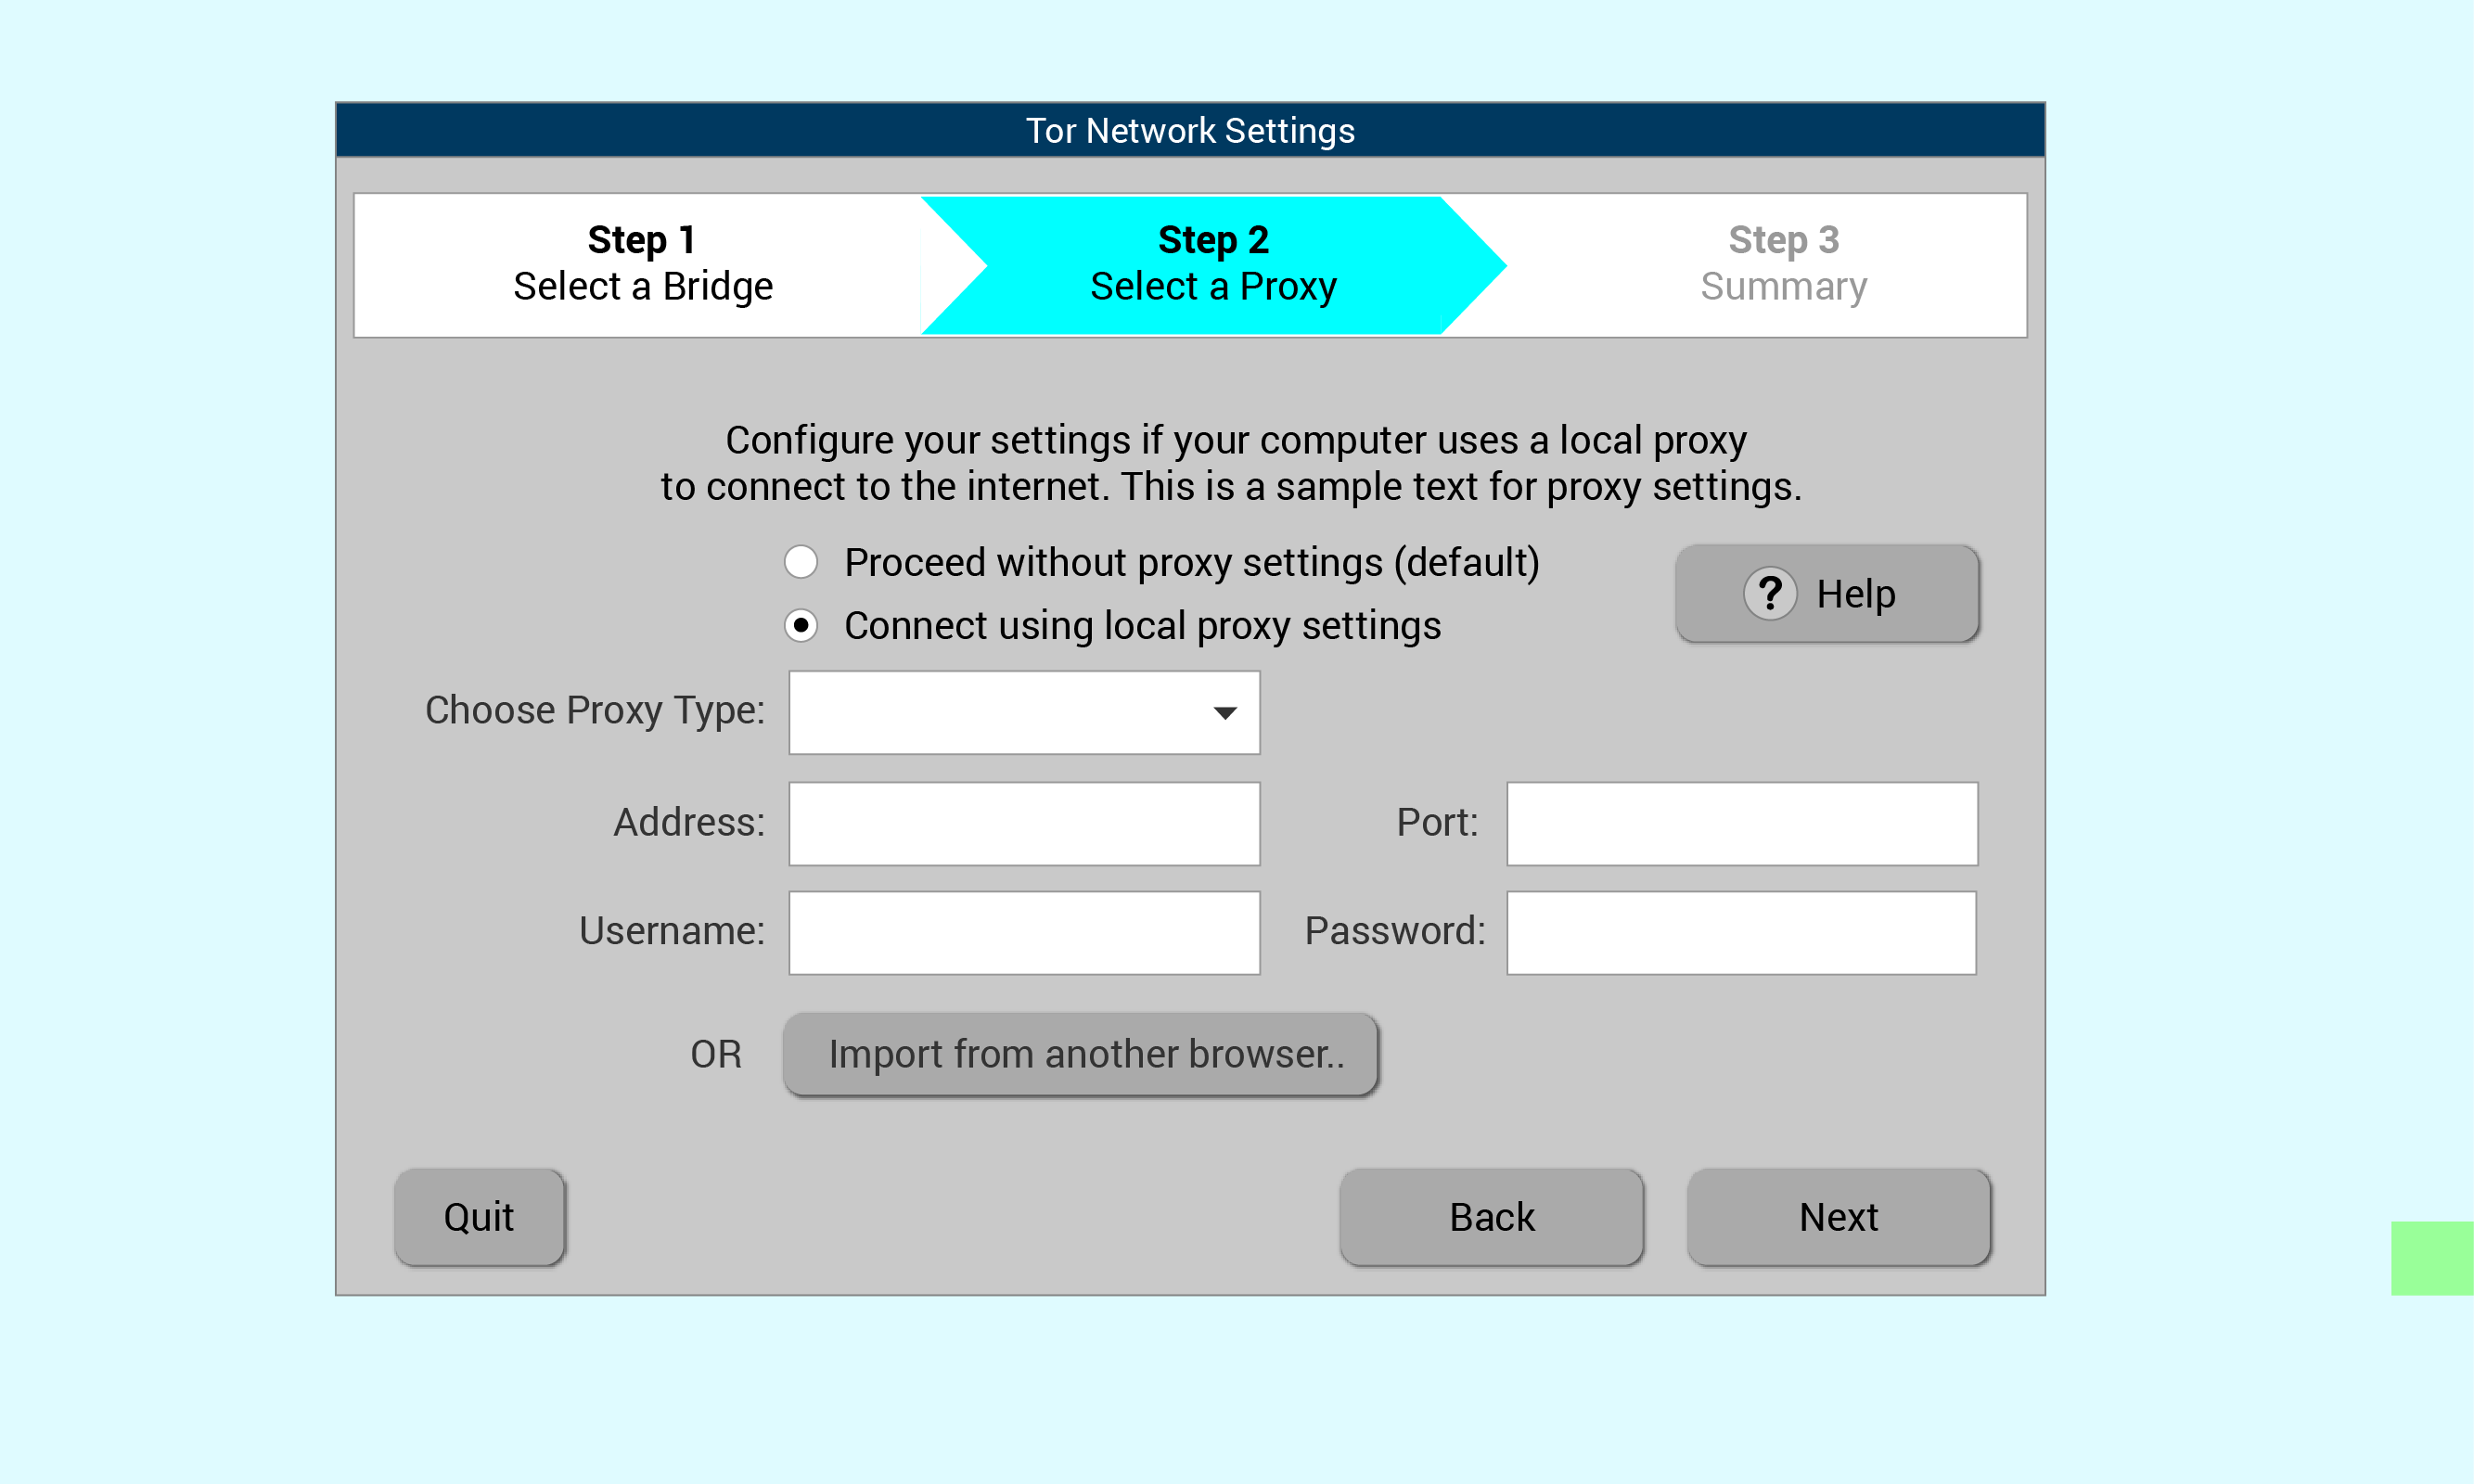
\includegraphics[width=0.5\textwidth]{redesign-proxy.png}
    \caption{the proxy configuration screen, with an option to automatically
        ``Import from another browser''}
\end{figure}

\noindent {\bfseries Building a better mental model}
Participants' lack of a mental model of censorship led them to believe their
Tor connection was censored when, in reality, it was not. It furthermore contributed
to their confusion between bridges and proxies. Our design directly addresses
these issues.

Potentially ambiguous text (i.e., referring to censorship) is removed in favor
of stating the underlying options, as it was shown to confuse our participants.
Previously, separate screens with binary options (Do you need a proxy? Yes/No) 
were provided to help users decide if they needed a bridge or proxy.
We have removed these screens
because our participants did not understand how to answer them correctly.

All information about bridges is now contained on one
screen in the interface, giving the user the full context of their decision.
The same is done with proxy settings.
The recommended option (choosing no bridge and no proxy) is now the default on
the respective configuration screens (Figure \ref{fig:redesign-noproxy}).
This results in a more streamlined interface with fewer windows
and fewer clicks required for our participants. \\

\begin{figure}[t]
\label{fig:redesign-noproxy}
  \centering
    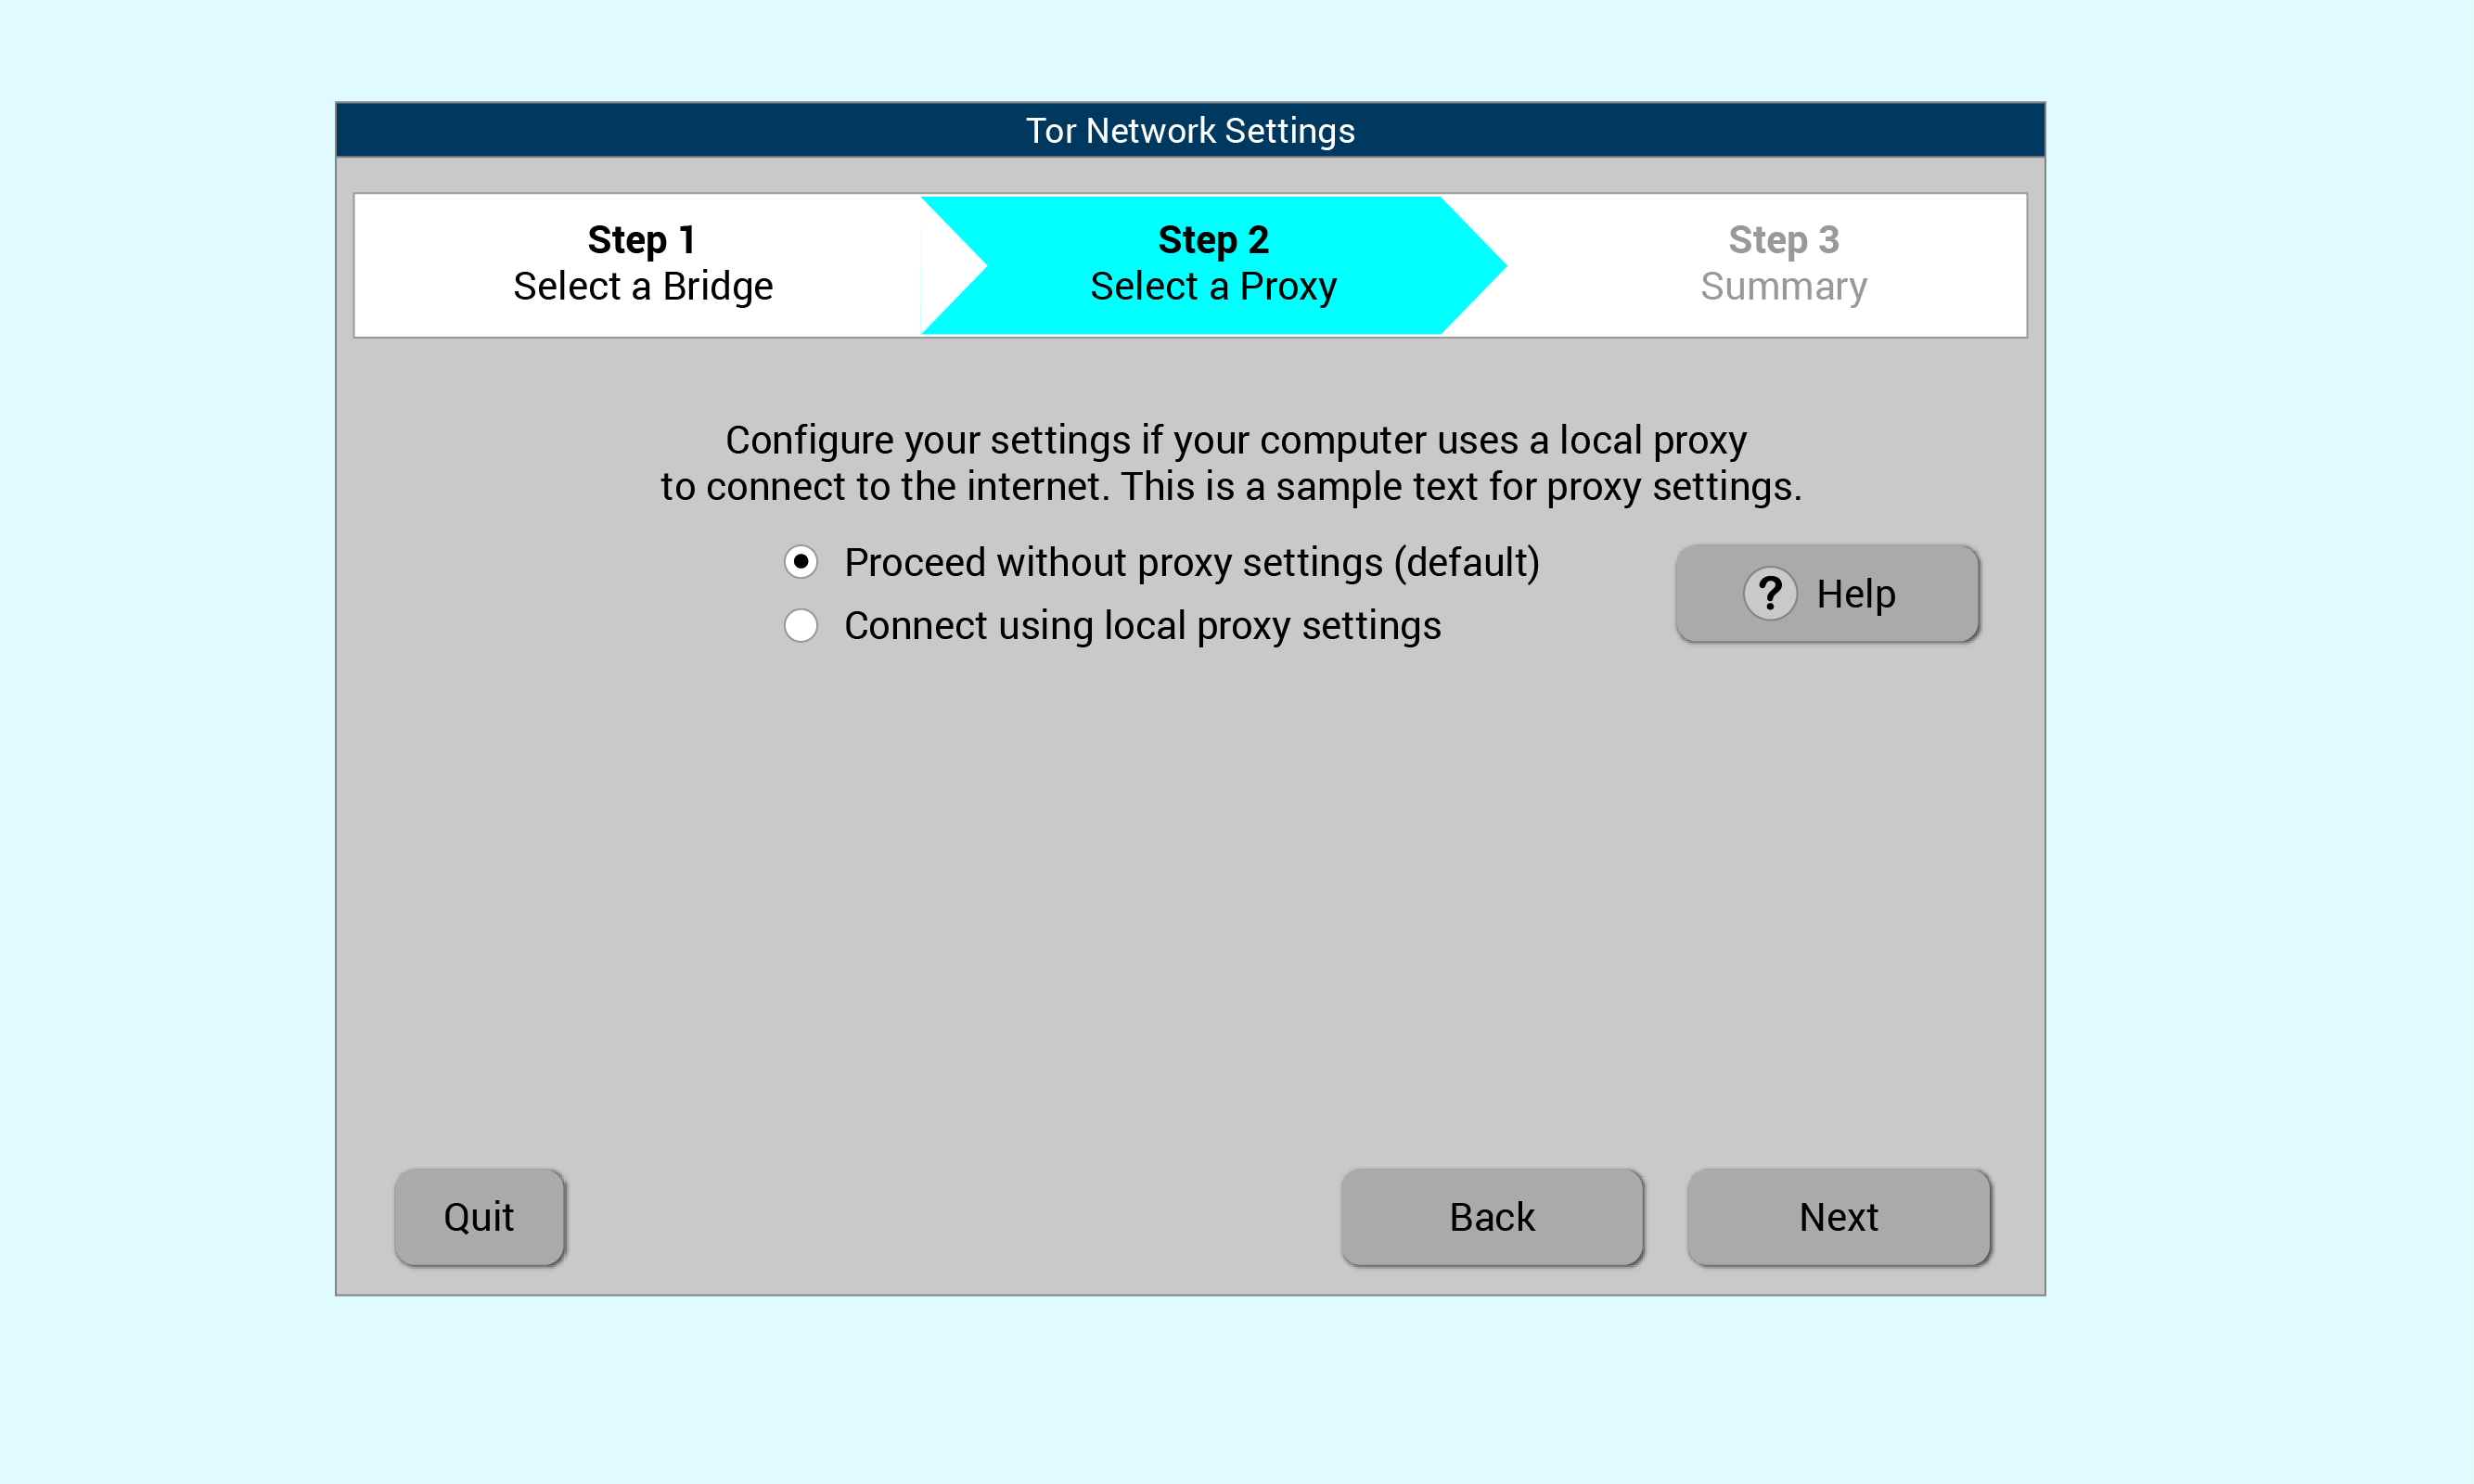
\includegraphics[width=0.5\textwidth]{redesign-noproxy.png}
    \caption{The default option is now to ``Proceed without proxy settings.''}
\end{figure}

\noindent {\bfseries Clarifying paths through the interface}
Many users struggled because the workflow implicitly suggested by the interface
didn't match the ideal path: crucial steps to follow were unclear or obscured,
while undue prominence was given to comparatively less important elements.
Our new design inverts this trend, focusing attention on the interface elements
that are more important, or more generally applicable.

A clear example of this is the ``Connect'' button on the first screen
(Figure \ref{fig:redesign-firstscreen}), which has
increased in size and become green, making it more prominent as the recommended
option. We believe that this will help the majority of Tor users. 
Although some of our participants in environments had chosen to connect
directly when they needed to configure,
the majority of censorship today can be circumvented with a direct connection. 
A similar aesthetic applies to the connect button seen after custom
configuration.

\begin{figure}[t]
\label{fig:redesign-firstscreen}
  \centering
    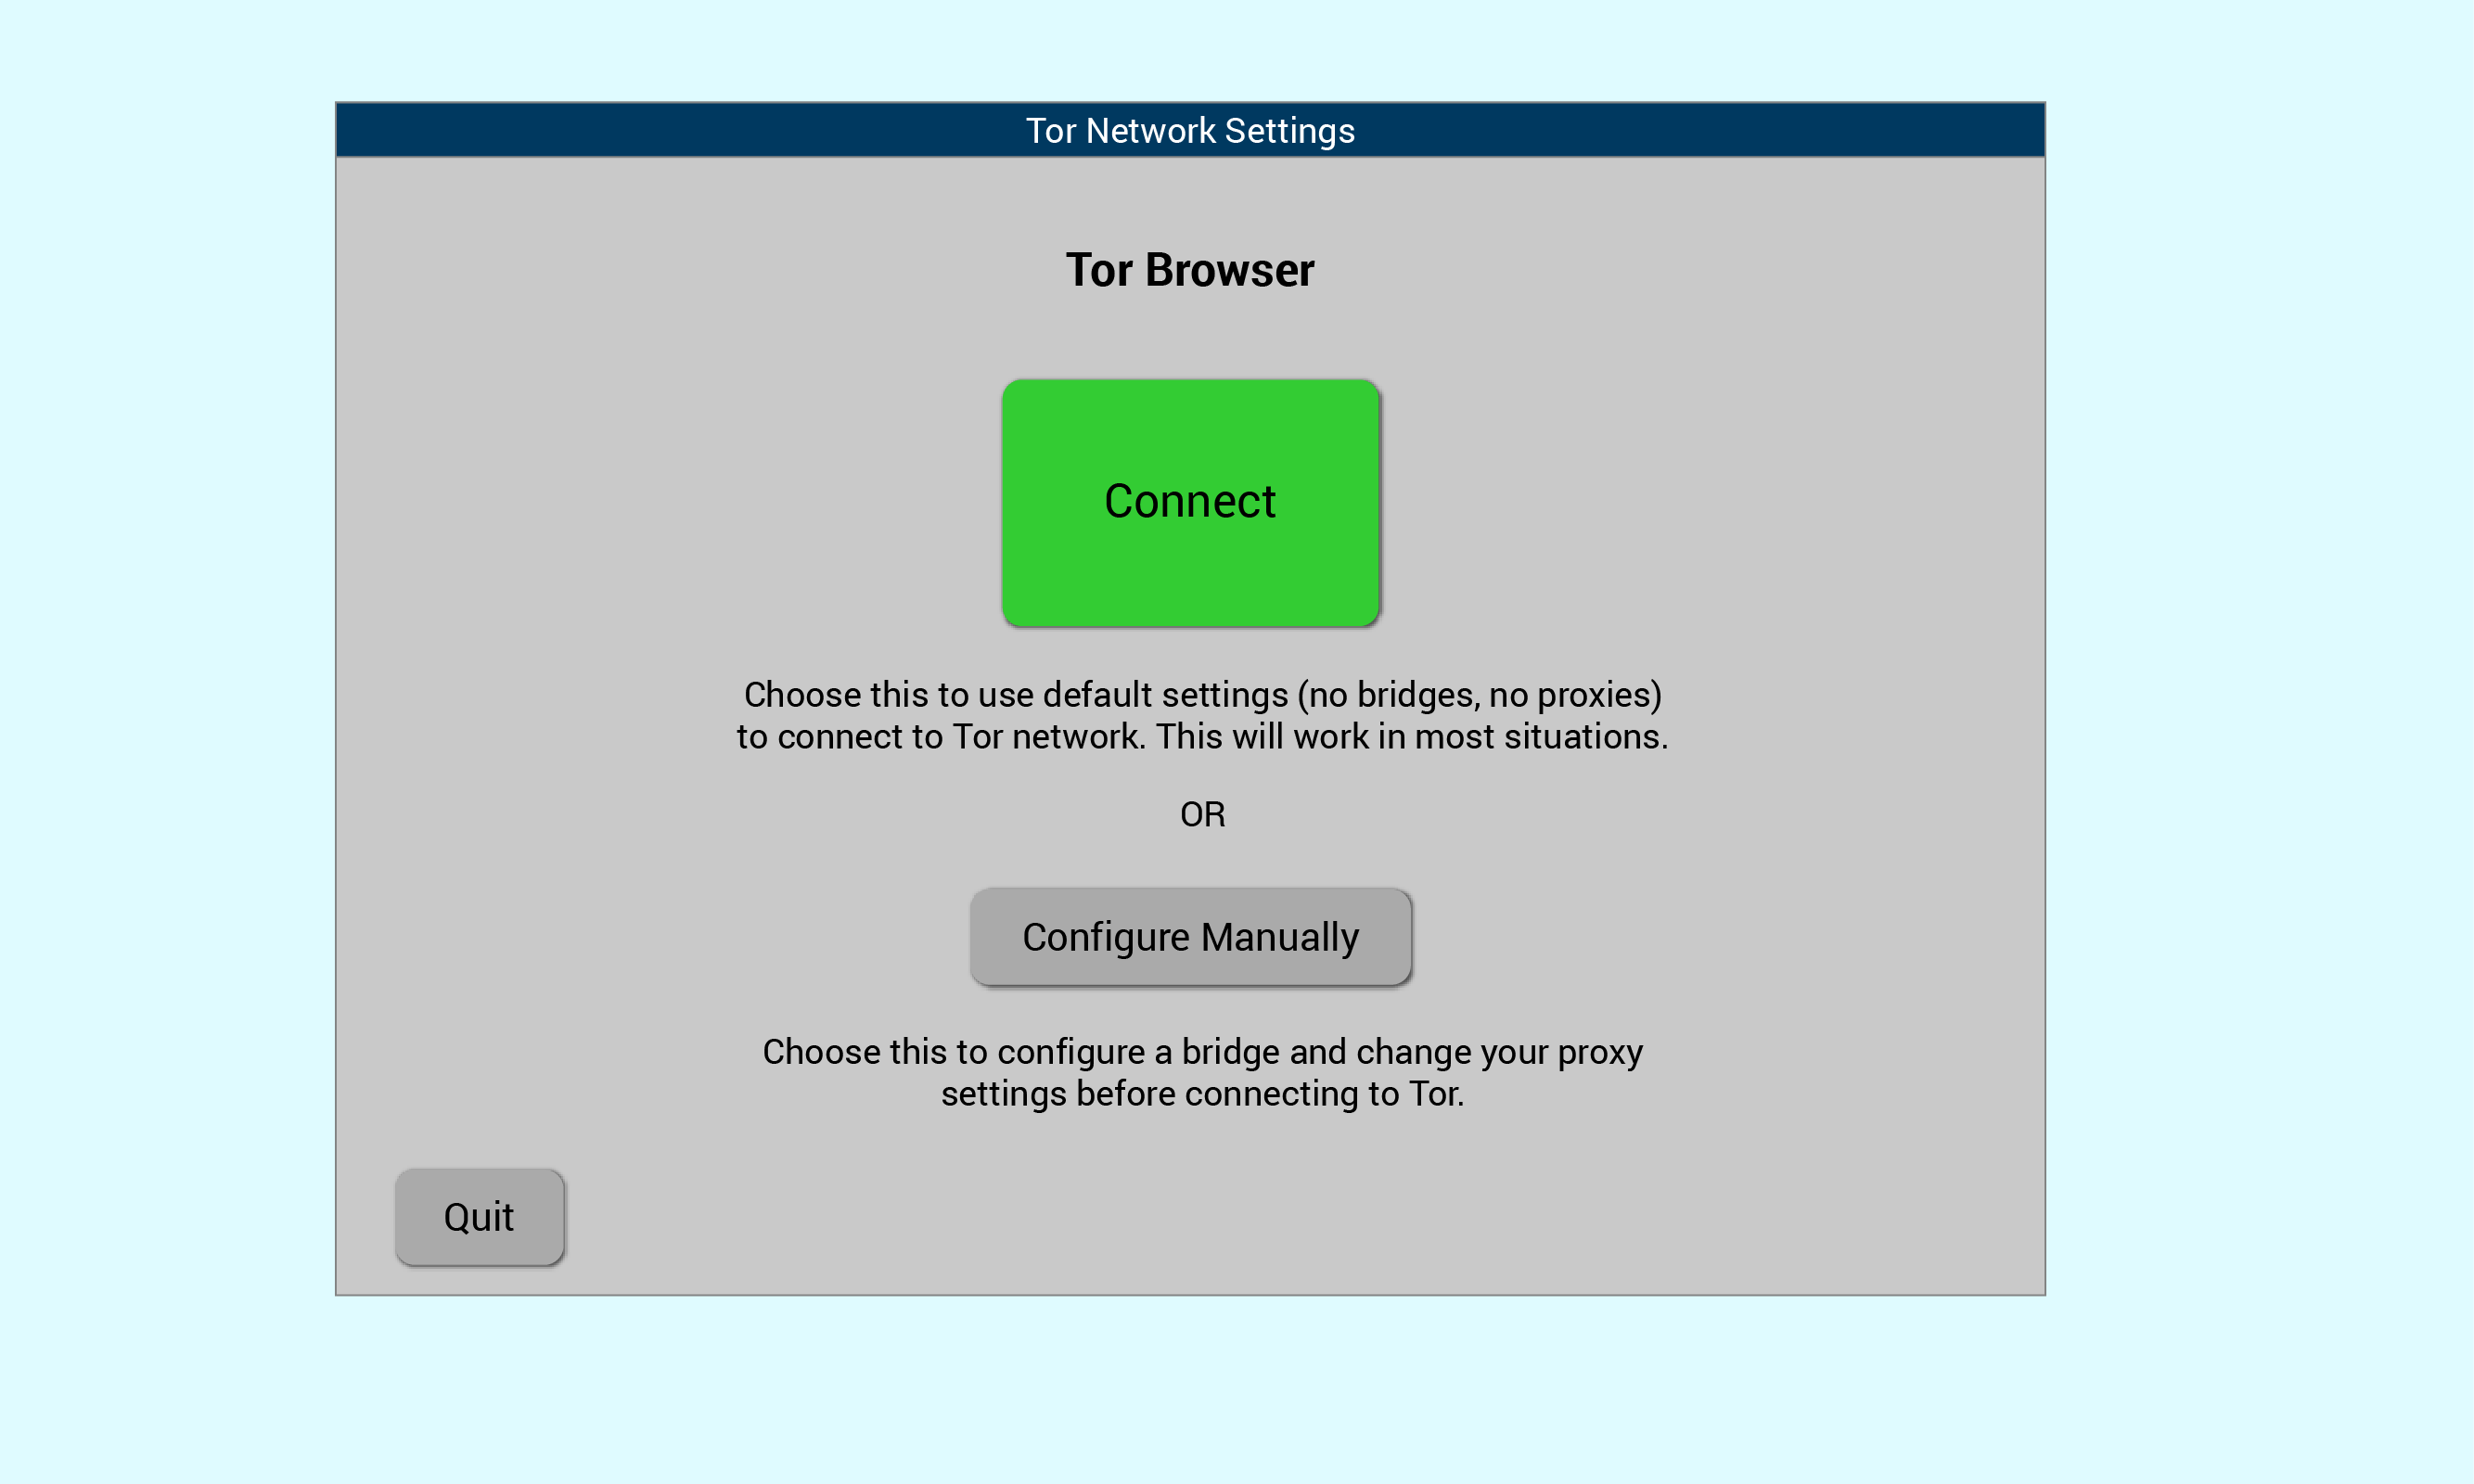
\includegraphics[width=0.5\textwidth]{redesign-firstscreen.png}
    \caption{the initial connection screen. Note the prominence given to the
    ``Connect'' button.}
\end{figure}

To help lessen the cognitive load and use a proportionate amount of space,
recommended options are selected by default, and rarely used
elements are deemphasized.
The help button on the bridge configuration screen
has been emphasized to be bigger, since it is a helpful option which people rarely
clicked. To discourage our users from using an advanced setting
that should only be used in very rare circumstances,
we have now incorporated the custom bridge configuration in the dropdown menu
(Figure \ref{fig:redesign-bridges});
it previously took up a significant portion of the bridge configuration screen. 

\begin{figure}[t]
\label{fig:redesign-bridges}
  \centering
    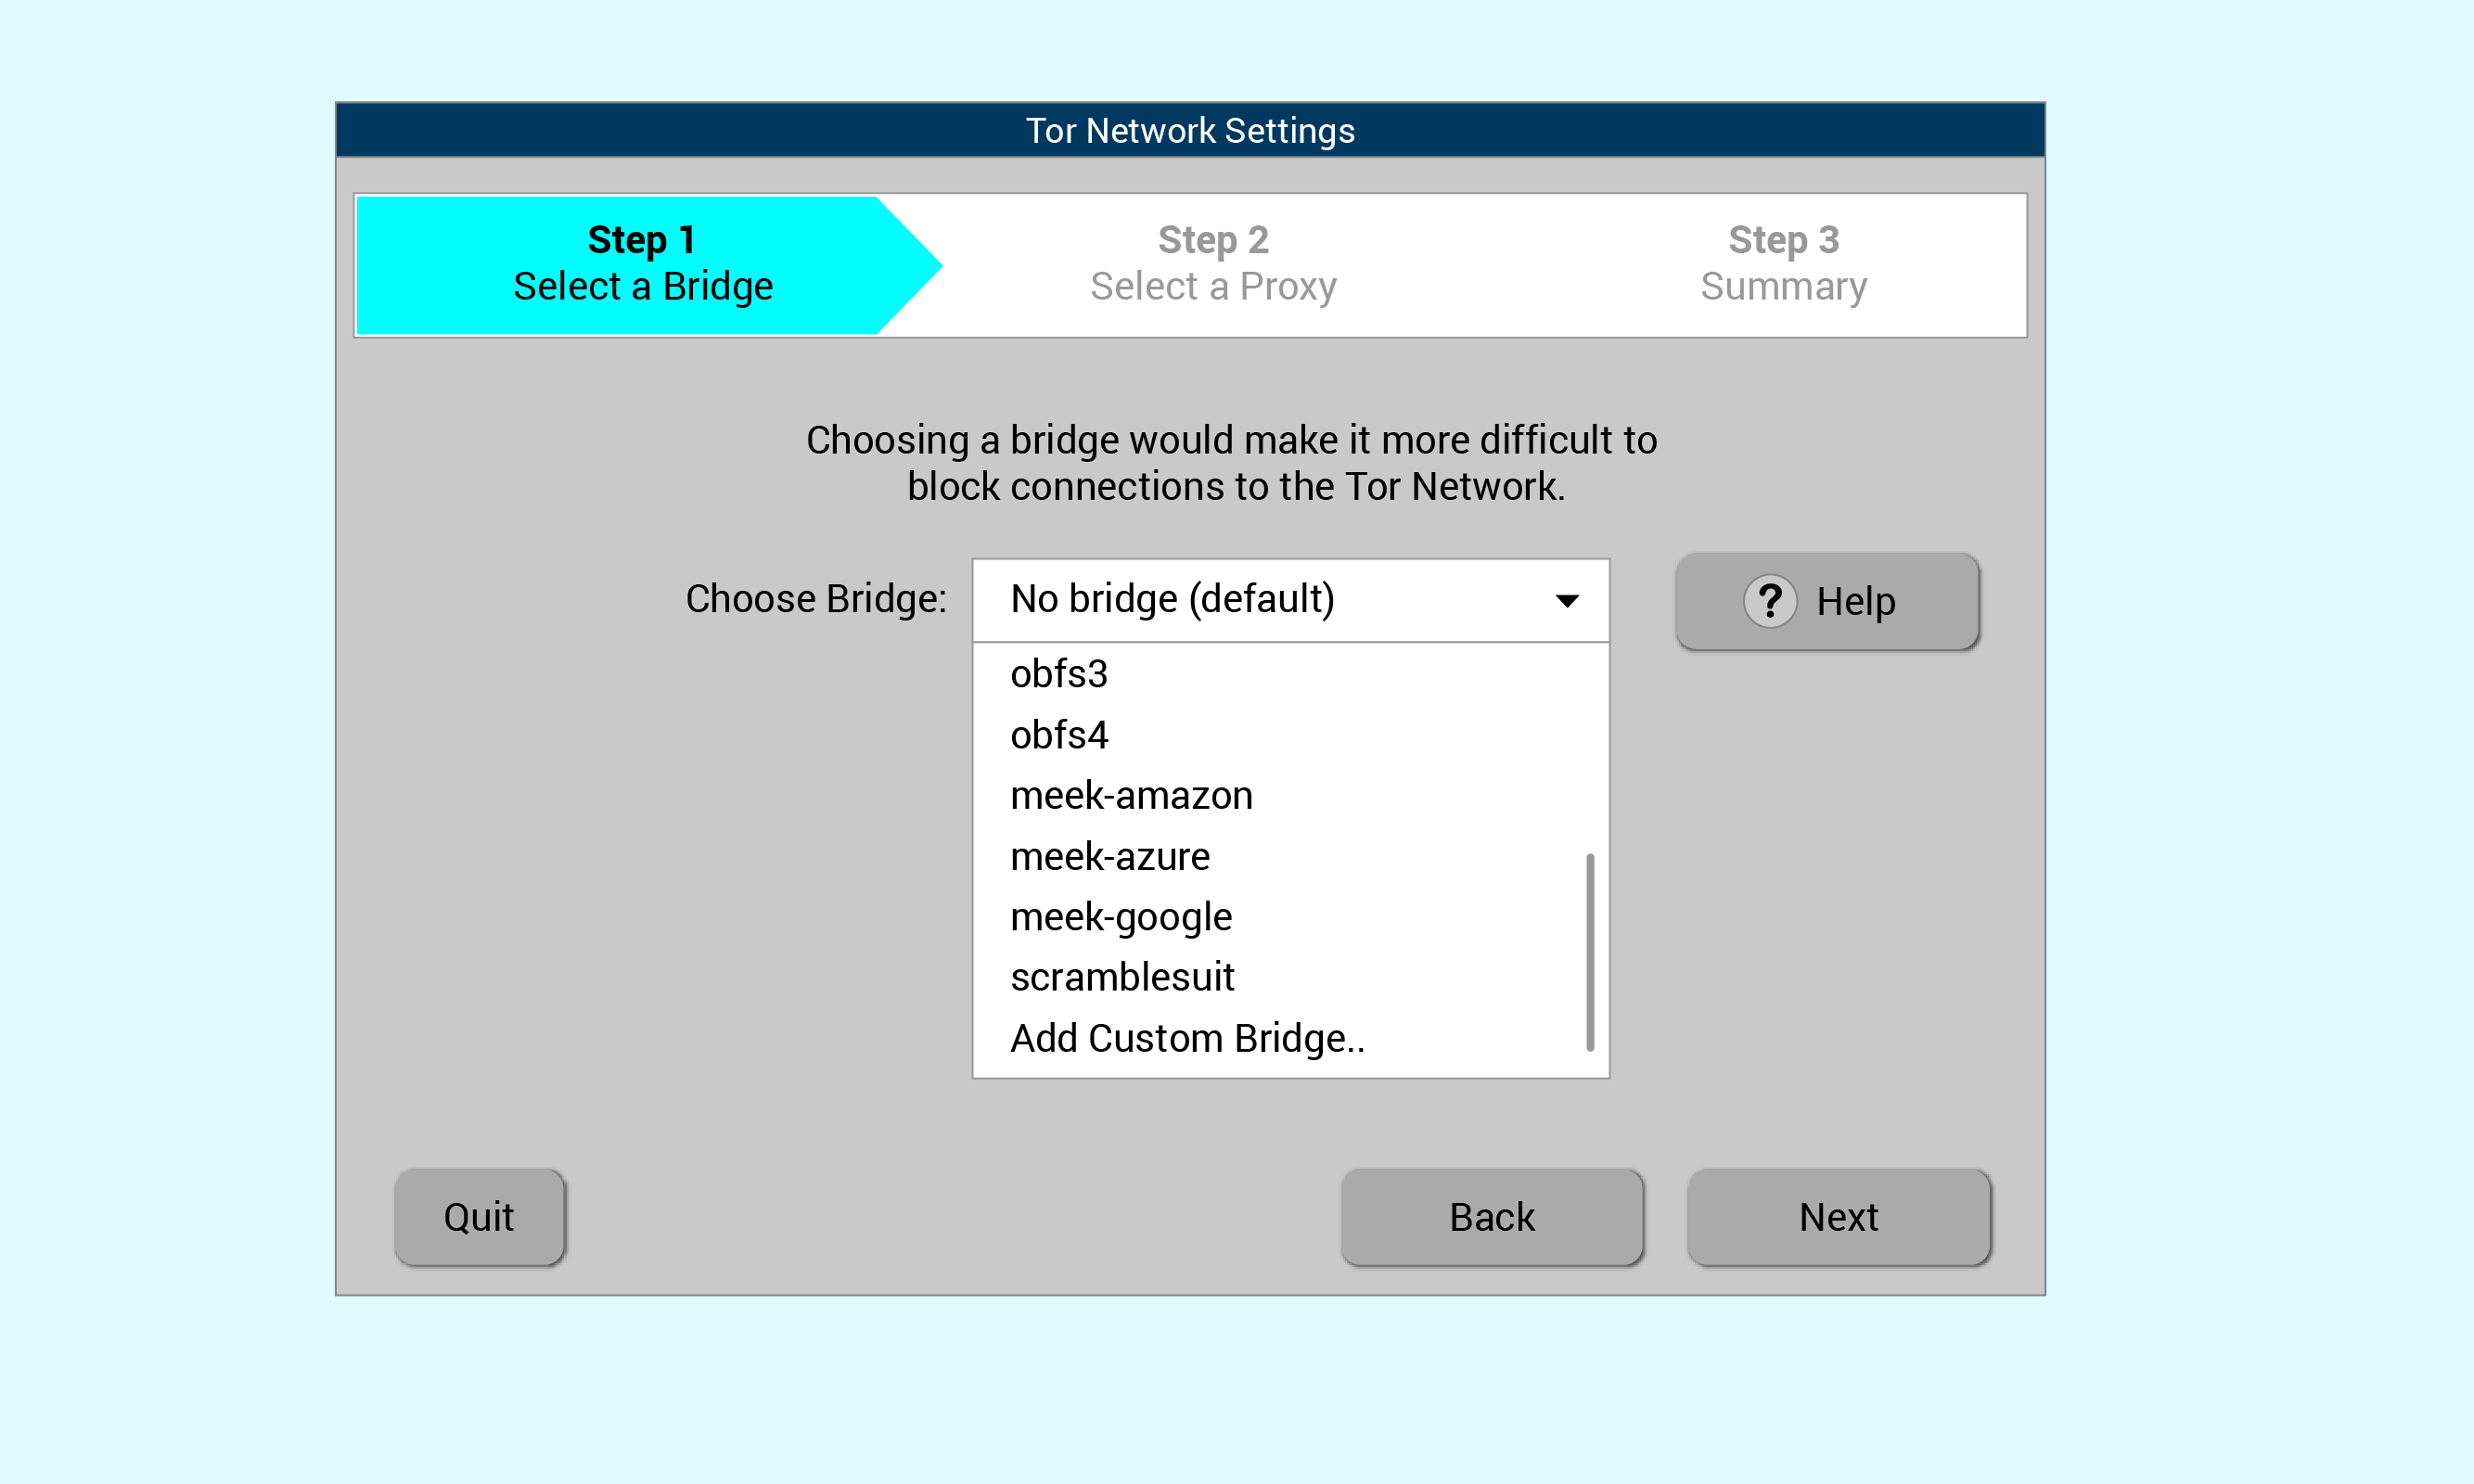
\includegraphics[width=0.5\textwidth]{redesign-bridges.png}
    \caption{the bridge selection screen, with the option to ``Add Custom
    Bridge''}
\label{fig:redesign-bridges}
\end{figure}

A progress indicator at the top of the window indicates various steps
for configuring a connection. In addition to communicating what the various 
steps of configuration are from the beginning, this indicator also serves to clarify the independence of
bridges and proxies, which need to be configured separately. 

After a failure, the users are
returned to the first step of the process -- the bridge configuration -- since this
is usually the cause for configuration issues. Previously,
the user had to manually click to go backward in the dialog to configure bridges.
In the rare event that the proxy is the issue for the connection setting, the user
will be directed to the proxy page naturally through the flow of the UI. \\

\noindent {\bfseries Designing for failure cases}

Users were led astray by interface elements that were unhelpful or
misleading if the program encountered connection problems. Our design seeks to
prevent such confusion by anticipating failures and providing specific instructions
for our participants on their next steps.

The progress bar in the connection window was often unresponsive
and did not offer guidance for how long users were supposed to wait.
The connection process can take about two minutes --- long enough that users may
think that the connection has failed, even when it is making slow and invisible progress. 
We added a countdown timer to indicate that a long wait time does
not indicate failure. We also add visual indicators
for major milestones in the connection, providing better feedback about what has
been accomplished so far. Additionally, the current status of the connection
attempt (drawn from the log) is displayed, to aid in understanding and
debugging.

\begin{figure}[t]
\label{fig:redesign-waiting}
  \centering
    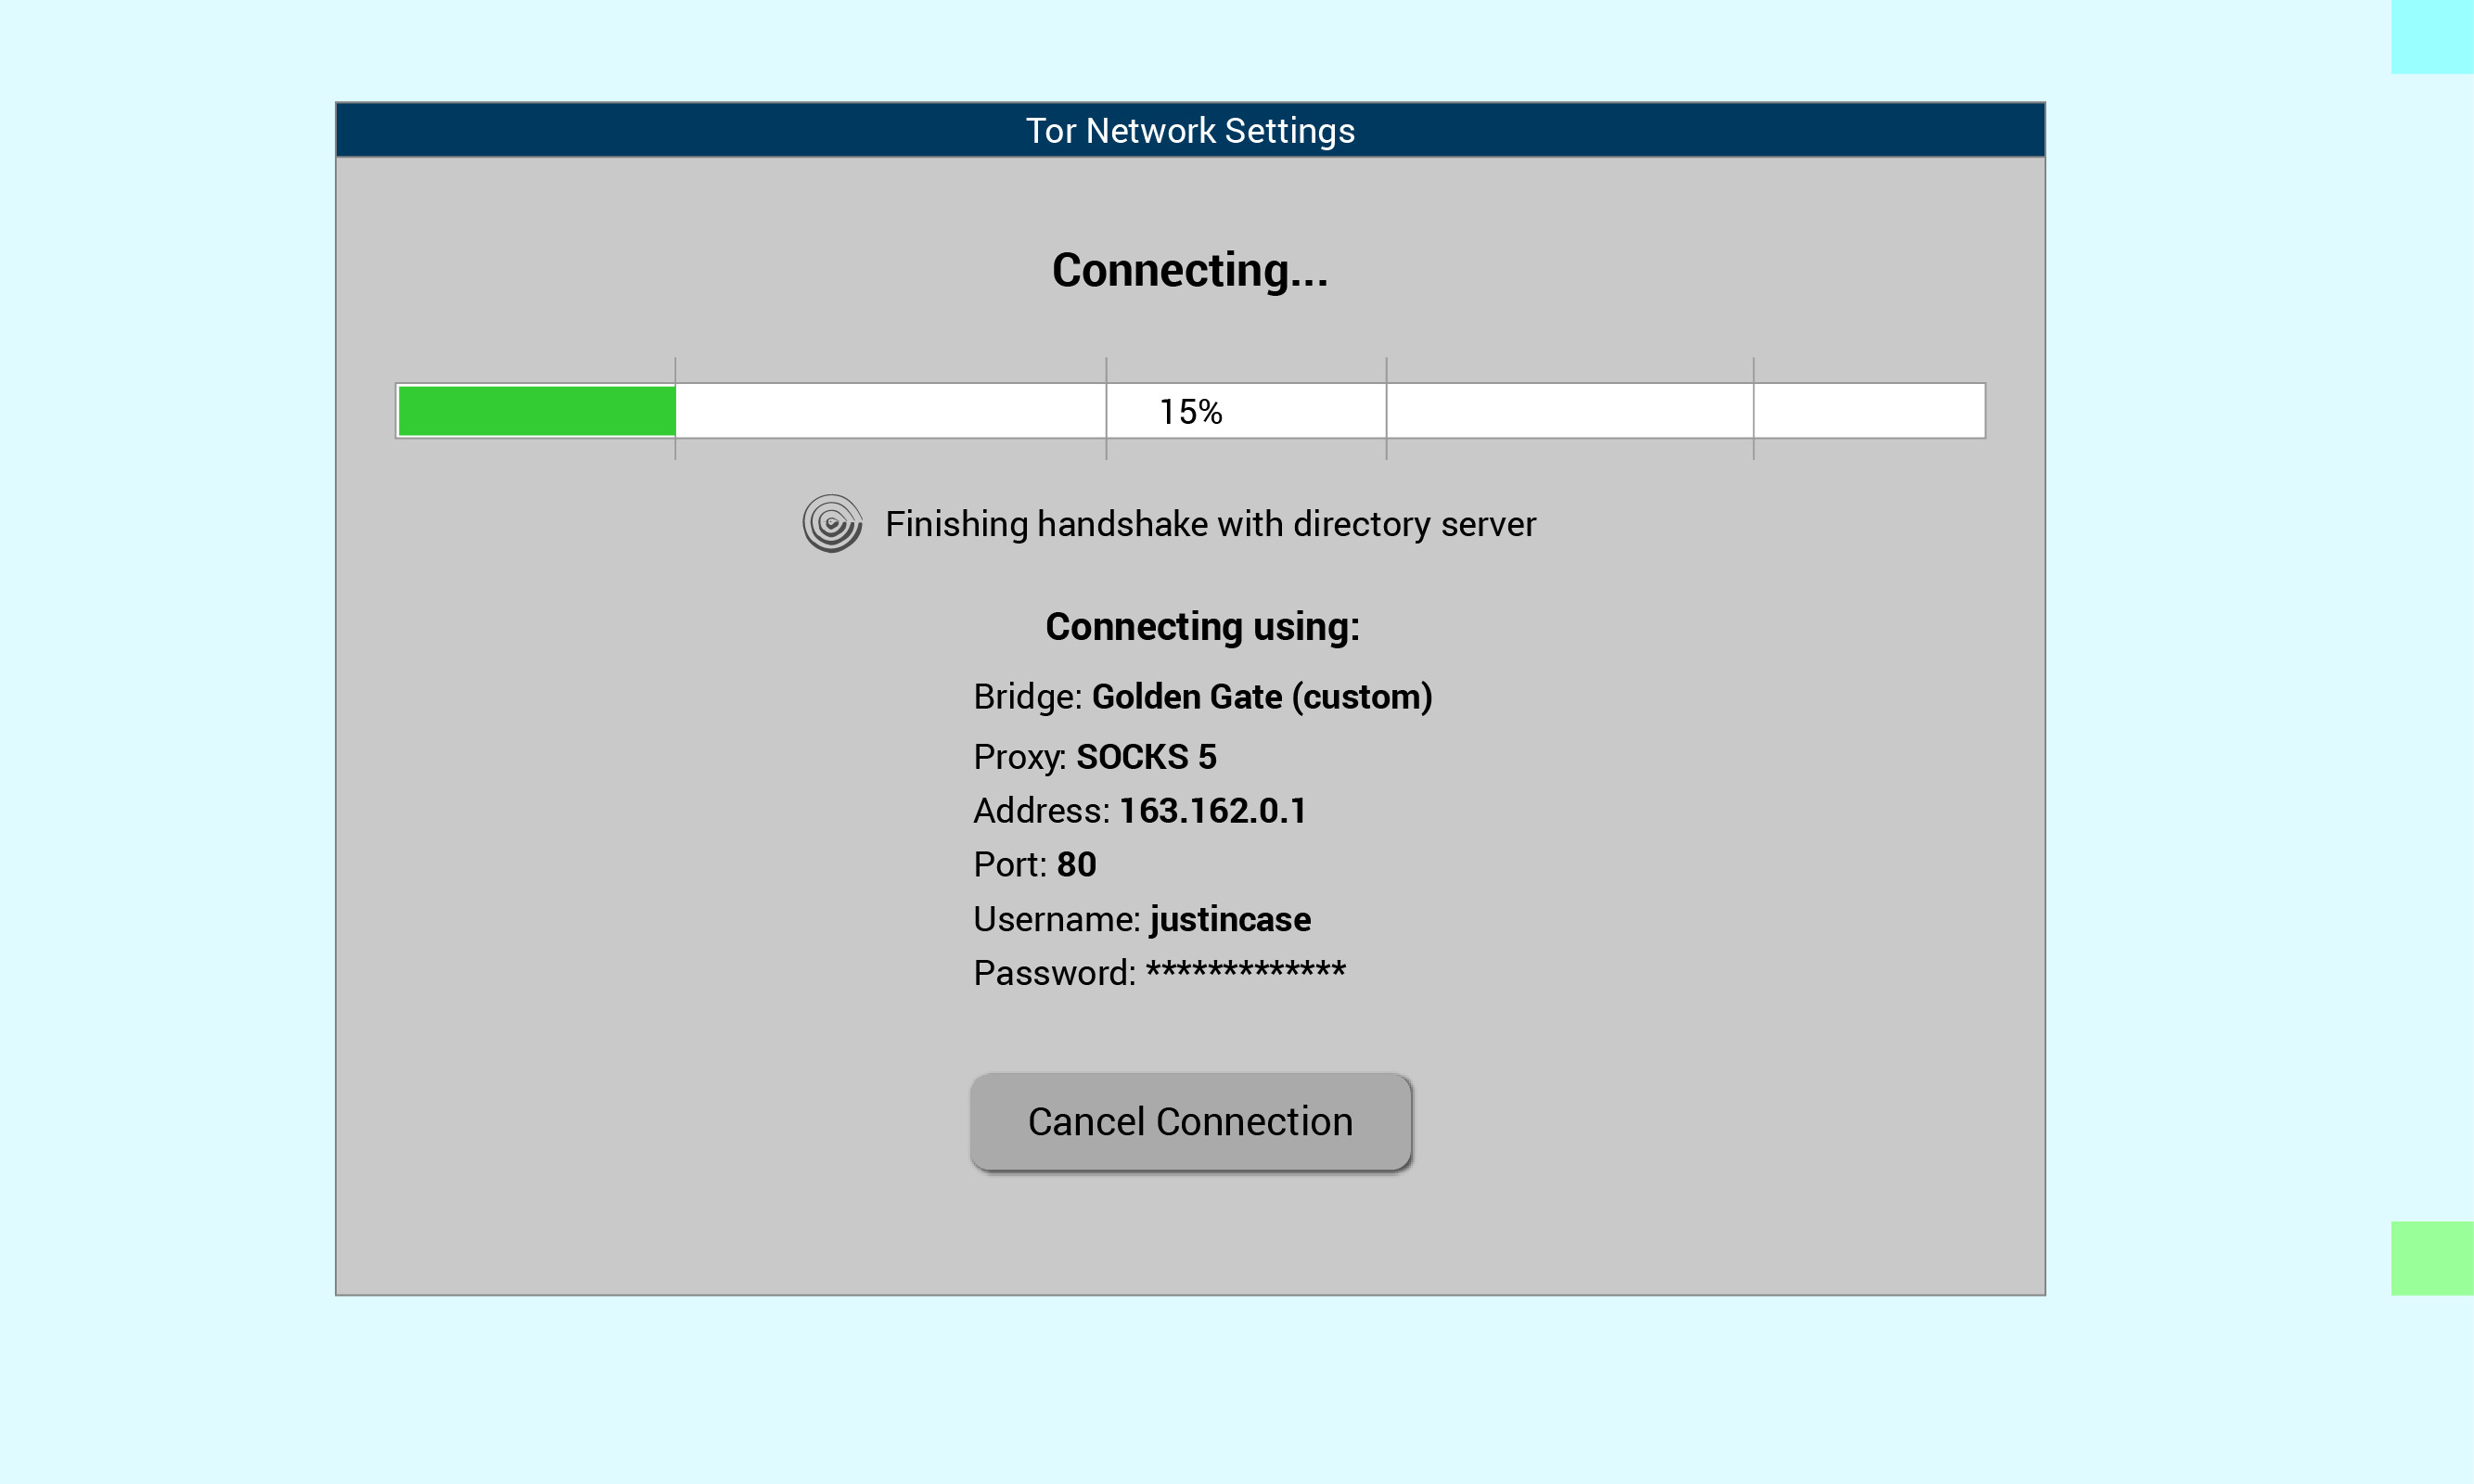
\includegraphics[width=0.5\textwidth]{redesign-waiting.png}
    \caption{the new connection screen}
\end{figure}

In the event that the connection attempt fails, messages from the log are
displayed, along with suggestions about what to do next (e.g., try
another bridge). To make the potential options clearer, the new failure screen
includes a separate button for common next steps which are able to resolve
a failed connection, which are to retry without changing settings and to reconfigure 
the connection. \\

\begin{figure}[t]
\label{fig:redesign-failure}
  \centering
    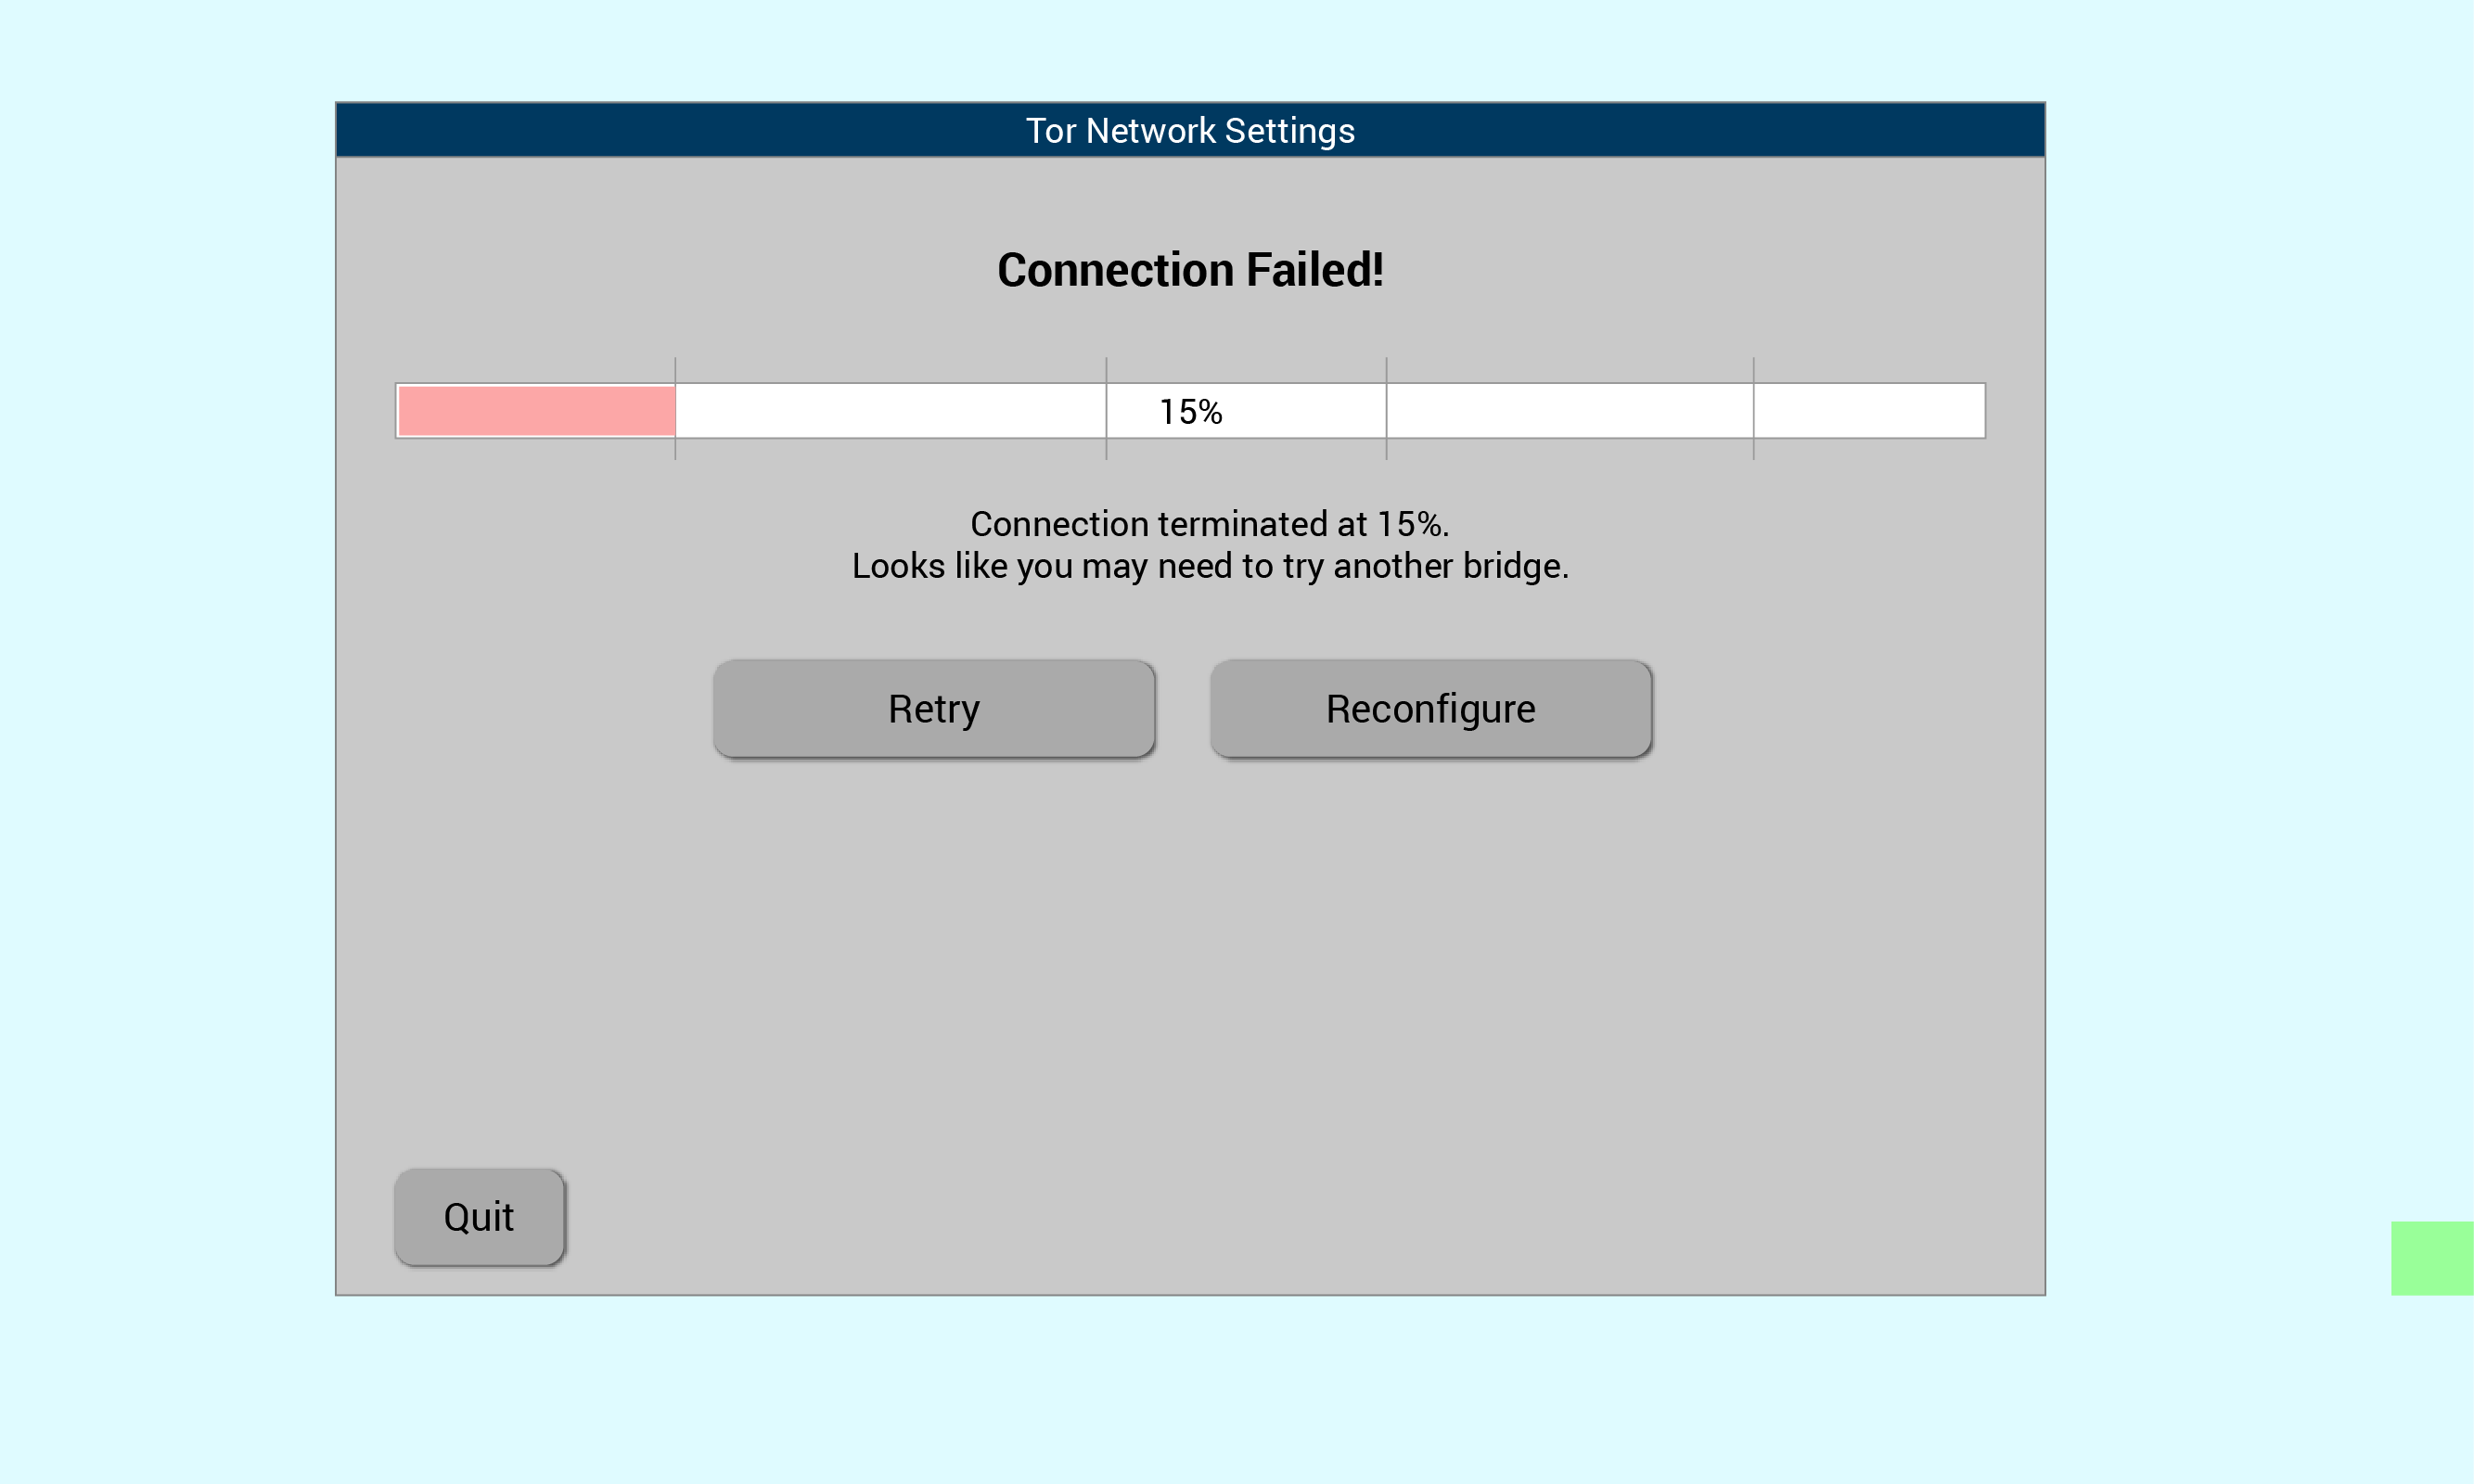
\includegraphics[width=0.5\textwidth]{redesign-failure.png}
    \caption{the screen displayed when a connection failed}
\end{figure}


\noindent {\bfseries Additional changes}
In addition to the changes above, we have simplified flows,
reduced text, and reduced visual clutter.
We believe these changes are cohesive with our design
and will be beneficial for the user.\\

\section{Quantitative Testing}
{\color {red} TODO}

\section{Evaluation}
{\color {red} TODO, write about what worked, what didn't, and what we recommend.}

\section{Discussion}
{\color {red} 
Talk about how the design was a conservative version. And why the conservative choices were made. For at-risk users, maintainability, etc.

Additional potential changes that could be made to the browser: 
\begin{itemize} \itemsep1pt \parskip0pt \parsep0pt 
\item {\bfseries Tell people to click connect.} On the first screen, there are no instructions for the user on what to do. There is a description of what each option means, but there is no guidance on what they should do. Ideally, we would people to click connect, and then try the manual configuration if a direct connection fails. But communicating this may put some users at risk. I would argue that the benefit is higher than the risk. 
\item {\bfseries Auto-configure after connect.} After a person has already clicked connect and the connection was unsuccessful, they have already been logged. I am assuming that the significant difference is between being logged trying to connect to Tor or not at all, rather than the number of connection attempts made. This would greatly save our users a lot of headache. 
\item{\bfseries Hide the proxy screen.} Don't give users the option to configure a proxy unless it has been detected that it would be necessary. The amount of people who use proxies is low, but then ... this would not give users control in the beginning of the configuration process. 
\item{\bfseries Ask about the risk.} Rather than having the configuration dialog be manual by default, just ask if the users are at risk if the process was automated. If they are not at risk, we can do it automatically, and the at-risk users can configure manually. The issue with this is that people may not answer this question honestly, or they might not know the correct answer to this question. 
\item{\bfseries Ask if they are qualified to make decisions.} Asking users if they know which bridge to choose, and choosing for them if they say they don't know. We probably know better than they do. But there are ethical implications of choosing bridges for them rather them making the mistakes themselves. The issue with this is that people may not answer honestly. 
\end{itemize}
}

\section{Future Work}

The work summarized is only a part of the process of improving the Tor configuration
dialog for more usable censorship circumvention. We plan to continue this work by:

\begin{itemize} \itemsep1pt \parskip0pt \parsep0pt 
\item {\bfseries Testing our design with a small-scale qualitative study.} It is
    critical to get in-depth data from users through one-on-one interviews and
    open-ended feedback. For this reason, we plan to run a small-scale
    qualitative study similar to the one we have run for the old interface. We
    plan to run these studies at the start of Spring 2016.
\item {\bfseries Testing our design with a large-scale quantitative study.} To
    test our design alongside the old interface, we will recruit a large number
    of participants to try out both designs. The purpose of this is to get
    statistically significant results on whether our design choices have helped
    users to configure successfully. We plan to run these studies at the start
    of Spring 2016.
\item {\bfseries Analyzing which design changes have made a positive impact.} We plan to instrument our interfaces to capture all clicks, window transitions, and other events so that we can analyze if our designs have helped our users connect faster and or with less effort. 
\item {\bfseries Push some changes.} We have the input and support of Tor developers
to improve this interface. Any improvements will be incorporated into the Tor Browser.
\end{itemize}

\noindent {\bfseries Quantitative experiment analyses} We want to show a statistically significant improvement in user effort for a successful connection. We believe that this can be measured with various factors such as time, clicks, etc. For this reason, we will specifically be collecting data about: the total number of participants who have successfully circumvented censorship, the number of connection attempts for a successful connection, how much time participants spent configuring before a successful connection, the number of windows traversed in the UI, the number of clicks made, if bridge and proxy configuration interfered with each other, and how many people try repeat configuration settings. 

One exciting analysis we will perform is to build a Markov model of the UI flow chart (Figure \ref{fig:markov} shows a simplified illustration). We believe that this will be helpful in communicating participant behavior in aggregate since it will show the change in the UI flow structure, as well as how participants decisions have changed (e.g., in the old interface, a participant in a censorship environment which does not block Tor has a 0.4 chance of choosing ``connect,'' whereas in the new interface, the probability is 0.6). We have other visualizations in mind to display all participants' window traversal at a glance (Figure \ref{fig:bar} shows a simplified illustration), as well as other analyses.\\

\begin{figure}[t]
  \centering
    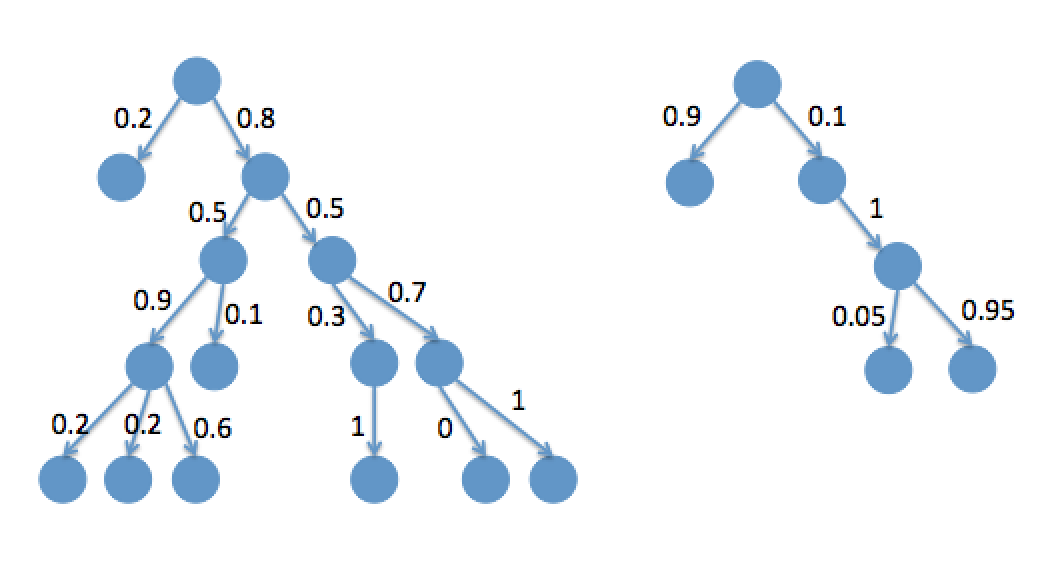
\includegraphics[width=0.5\textwidth]{markov.png}
    \caption{An illustration on a planned analysis using the quantitative survey data. This illustration shows two possible user interfaces and uses a Markov model to reflect the aggregate user behavior. We believe that this will be an concrete way to predict user behaviors, which is valuable feedback for if the interface is guiding users in a desired UI path.}
\label{fig:markov}
\end{figure}

\begin{figure}[t]
  \centering
    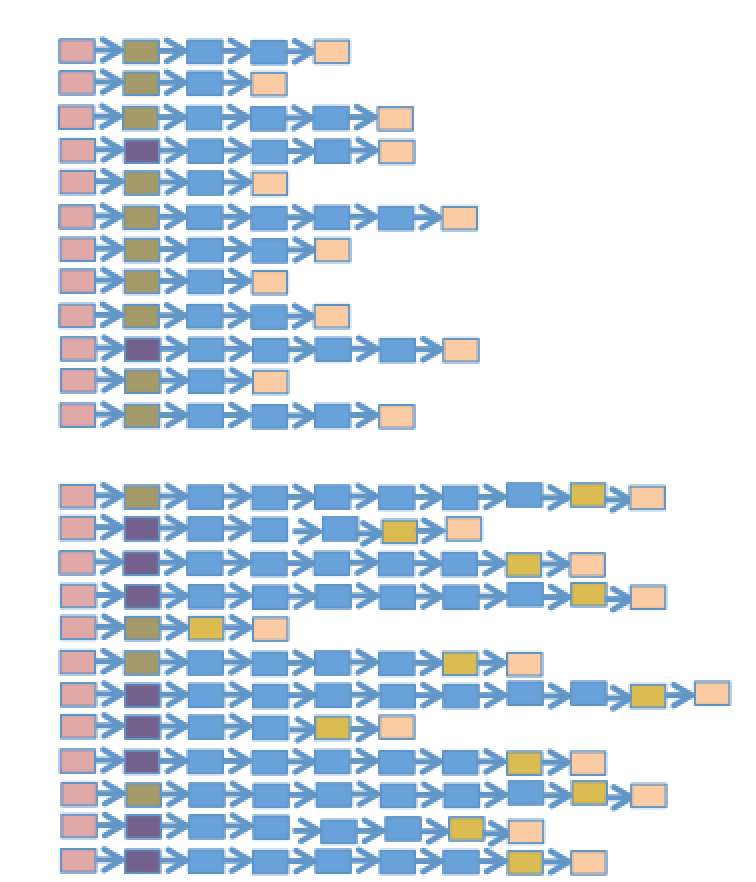
\includegraphics[width=0.5\textwidth]{screen-bar.png}
    \caption{An illustration of how we plan to visualize large-scale UI flows as a succinct way to display all participants' window traversal. We plan to color code the screens so that the reader can see trends at a glance, such as how the UI path for participants in a mild censorship environment with the old design compare to the UI flow for the participants in a mild censorship environment with a new design. It also can communicate how much work was required of a user to configure a connection.}
\label{fig:bar}
\end{figure}

\noindent {\bfseries Deciding which design choices to incorporate} We have discussed how we will decide if a design change is beneficial enough to incorporate. Intuitively, changes which lead to higher success rates, faster time to completion, less clicking, less window traversal, and positive changes in behavior will be incorporated. If they have the converse of these effects, those changes will not be incorporated. However, when changes do result in a statistically significant improvement or challenge, we have chosen to incorporate changes if they provide cohesion with other changes which do have positive effects. If changes seem to be uncorrelated to positive effects and do not show statistical significance, we will not incorporate those changes. \\

\noindent {\bfseries s} We will help incorporate changes into the Tor Browser. Since we have developer support, it is not expected that we implement our changes, but we will advise them on any changes that they make. We hope that our work is able to help people more easily access the free Internet. 

\section{Resources}
\noindent Our online artifacts of the work done during this class, Fall 2015,
are below: 
\begin{itemize} \itemsep1pt \parskip0pt \parsep0pt
\item \href{https://github.com/lindanlee/circumvention-ux-tor}{github repo with experiment plans, code, videos, interviews, and much more}
\item \href{https://marvelapp.com/15a2294}{a clickable prototype of our interface redesign}
\item \href{https://github.com/lindanlee/circumvention-ux-tor/tree/master/sessions/pre/videos}{qualitative interface evaluation videos}
\item \href{https://github.com/lindanlee/circumvention-ux-tor/blob/master/sessions/pre/participant-summaries.txt}{summaries of qualitative interface evaluation videos}
\item \href{https://github.com/lindanlee/circumvention-ux-tor/tree/master/sessions/pre/notes}{qualitative interface evaluation interview notes}
\item \href{https://github.com/lindanlee/circumvention-ux-tor/blob/master/setup/setup-environment}{experimental setup code: firewall and screen capture} 
\item \href{https://github.com/lindanlee/circumvention-ux-tor/blob/master/setup/takedown-environment}{experimental takedown code: saving files and cleanup} 
\end{itemize}

% from anonymity study
%Our online artifacts of study of Tor as an anonymity tool, such as 
%the summary, results, and resulting browser changes are below:
%\begin{itemize} \itemsep1pt \parskip0pt \parsep0pt
%\item \href{https://trac.torproject.org/projects/tor/wiki/org/meetings/2015UXsprint}{blog post summary}
%\item \href{https://blog.torproject.org/blog/ux-sprint-2015-wrapup}{changes made to Tor}
%\item \href{https://people.torproject.org/~dcf/uxsprint2015/}{subtitled screen videos}
%\end{itemize}

\bibliographystyle{abbrv}
\bibliography{circumvention-experiment.bib} 

\appendix
\section*{A1: Configuration Interface Windows}

\begin{figure}[h]
  \centering
    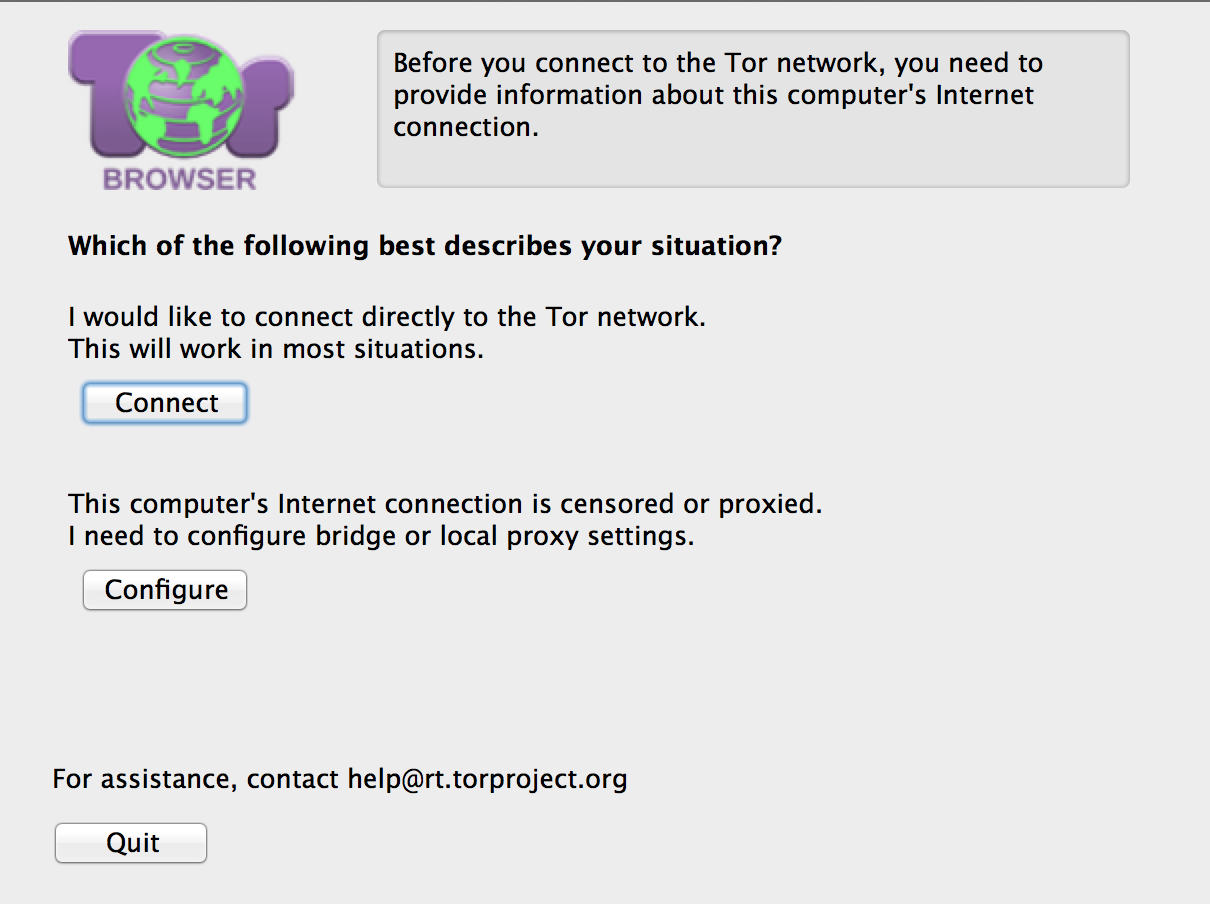
\includegraphics[width=0.5\textwidth]{window1.png}
    \caption{Window 1: the first configuration window shown to the user upon
    starting Tor Browser for the first time. Note that the interface's default choice
    is to connect directly through Tor. The interface also gives additional guidance
    to help users answer this question.}
\label{fig:window1}
\end{figure}

\begin{figure}[h]
  \centering
    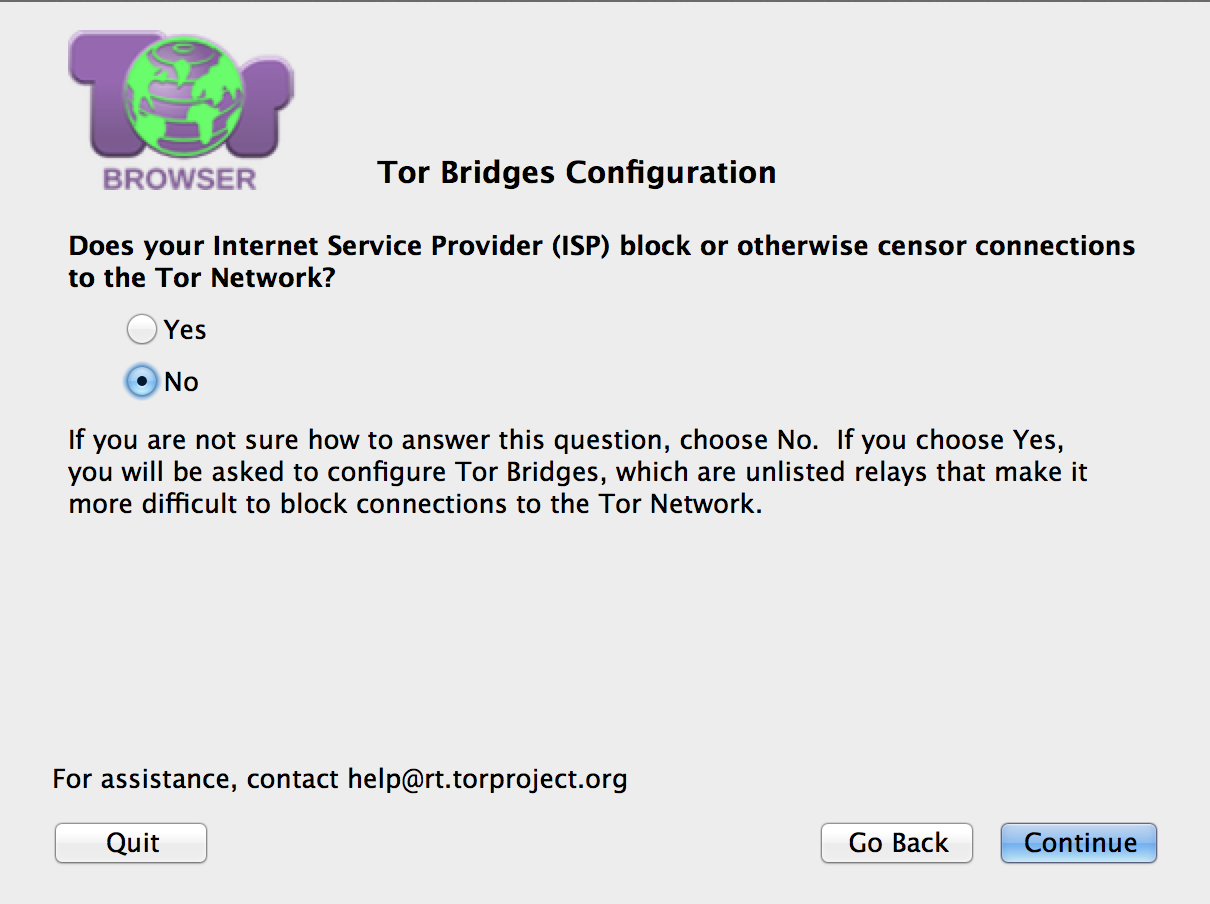
\includegraphics[width=0.5\textwidth]{window2.png}
    \caption{Window 2: This is the next window shown if a user chooses to configure 
    bridges or proxies. Note that the interface's default answer is ``No,'' 
    and also advises users to click ``No'' if they are unsure. The user can navigate to the 
    previous window by clicking ``Go Back,'' and continue configuration by clicking 
    ``Continue.''}
\label{fig:window2}
\end{figure}

\begin{figure}[h]
  \centering
    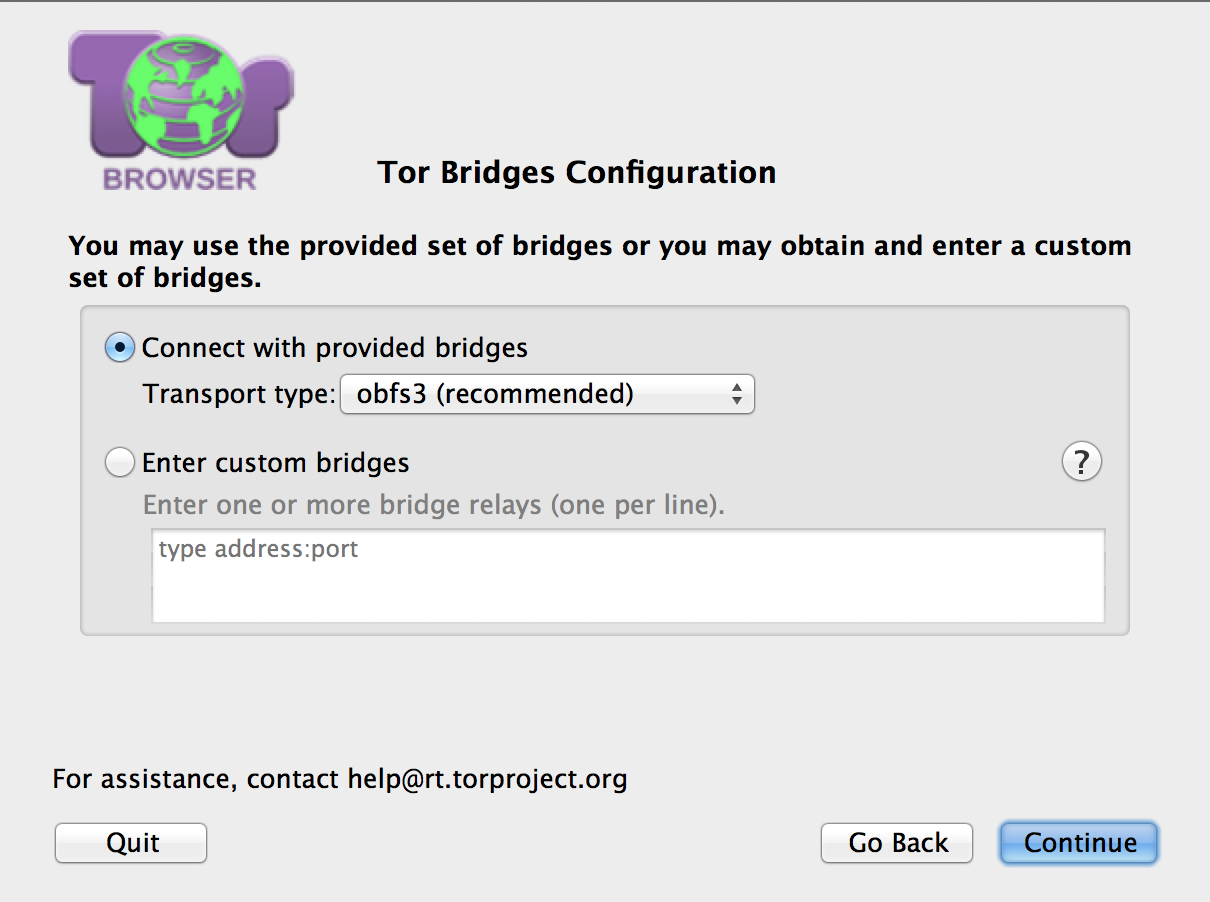
\includegraphics[width=0.5\textwidth]{window3.png}
    \caption{Window 3: This is the window shown when a user answers that a bridge 
    is required for the connection. Note that the default answer is to connect with a hard-
    coded bridge rather than to enter in a custom bridge, and to use the recommended 
    transport (obfs3). A possible source of confusion is that that the user is asked to choose 
    a transport type, when the interface clearly is asking for bridge configuration. The user 
    can navigate to the previous window by clicking ``Go Back,'' and continue configuration 
    by clicking  ``Continue.''}
\label{fig:window3}
\end{figure}

\begin{figure}[h]
  \centering
    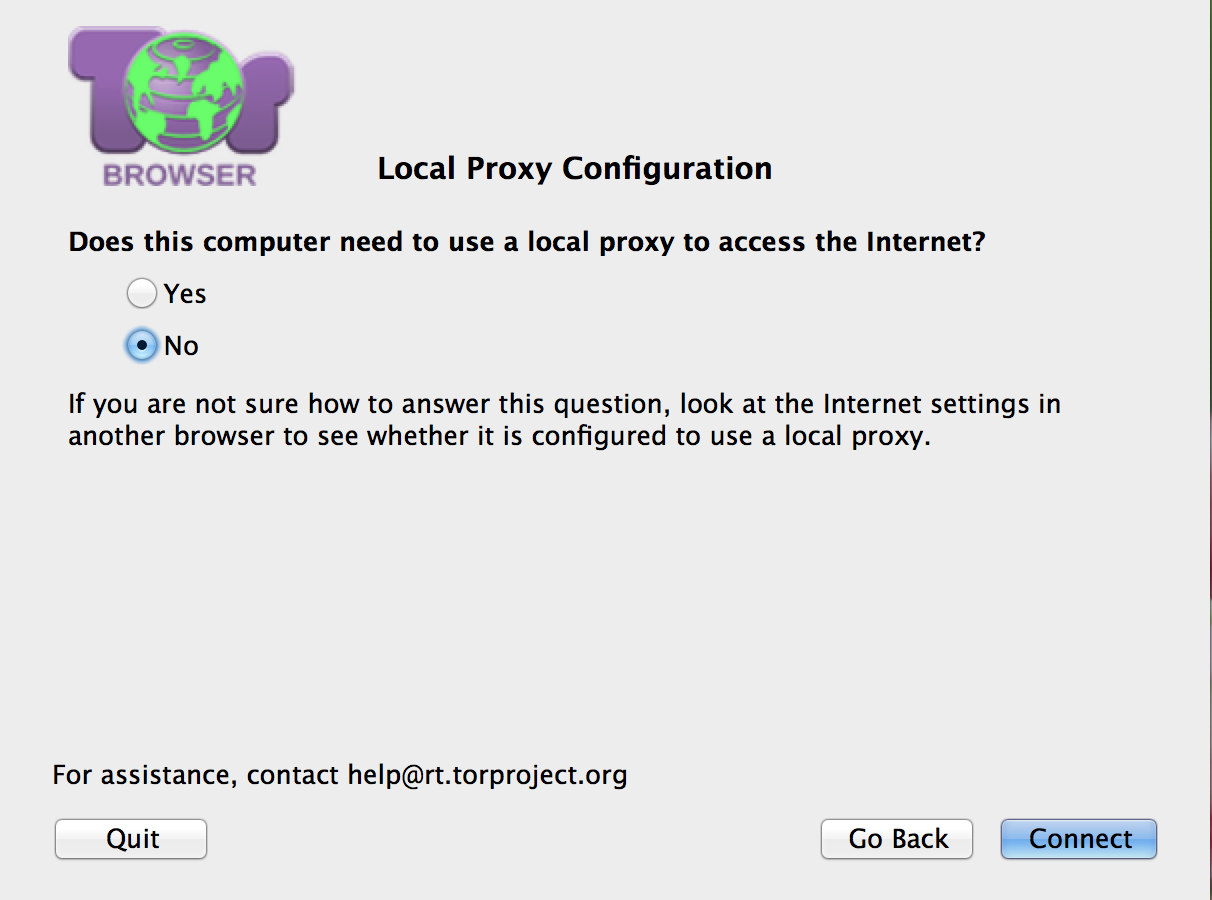
\includegraphics[width=0.5\textwidth]{window4.png}
    \caption{Window 4: This is the window shown after a user has deemed that a bridge
    is not required for the connection, or when the bridge configuration settings have been 
    chosen. Note that the default answer to if the user requires a proxy is ``No.'' Additionally,
    there is text to guide the users on how to answer this question. The user 
    can navigate to the previous window by clicking ``Go Back,'' and continue configuration 
    by clicking  ``Continue.''}
\label{fig:window4}
\end{figure}

\begin{figure}[h]
  \centering
    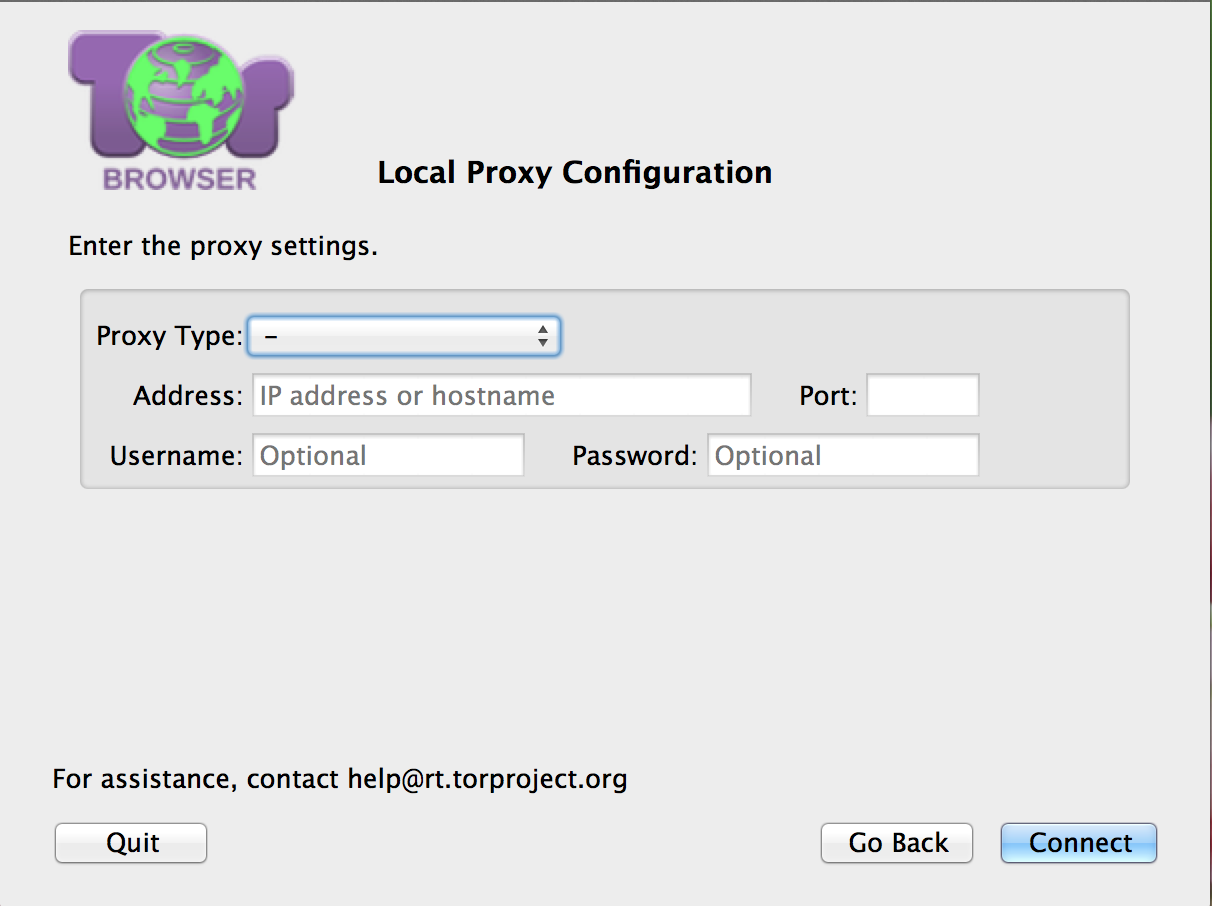
\includegraphics[width=0.5\textwidth]{window5.png}
    \caption{Window 5: This is the window shown when a user answers that a proxy is 
    required for the connection. Note that there are no default values in the answers, 
    where there were for bridges. Additionally, since this is the last window in the configuration
    interface, the options to navigate to other windows are to simply ``go back,'' or to 
    connect to the Tor Network.}
\label{fig:window5}
\end{figure}
\end{document}
